%==============================================================================
% AI6127 Group 13 -- 报告中文对照版（仅供组内阅读，不用于提交）
% 结构、编号、数字与英文版 main.tex 一一对应。
% Build:  latexmk -xelatex main_zh.tex
%==============================================================================
\documentclass[10pt,twocolumn,a4paper]{article}

\usepackage[a4paper,margin=0.75in,columnsep=0.25in]{geometry}
\usepackage{newtxmath}
\usepackage{fontspec}
\setmainfont{texgyretermes}[Extension=.otf, UprightFont=*-regular, BoldFont=*-bold,
  ItalicFont=*-italic, BoldItalicFont=*-bolditalic]
\setsansfont{texgyreheros}[Extension=.otf, UprightFont=*-regular, BoldFont=*-bold,
  ItalicFont=*-italic, BoldItalicFont=*-bolditalic, Scale=MatchLowercase]
\setmonofont{texgyrecursor}[Extension=.otf, UprightFont=*-regular, BoldFont=*-bold,
  ItalicFont=*-italic, BoldItalicFont=*-bolditalic]
\usepackage{xeCJK}
\setCJKmainfont{Songti SC}[BoldFont={Songti SC Bold}, ItalicFont={Songti SC}, ItalicFeatures={FakeSlant=0.18}]
\setCJKsansfont{Heiti SC}
\setCJKmonofont{Heiti SC}
\xeCJKsetup{CJKecglue={\hskip 0.15em plus 0.05em}}
\linespread{1.12}

\usepackage[table]{xcolor}
\usepackage{graphicx}
\usepackage{booktabs,tabularx,array,multirow}
\usepackage[group-separator={,},group-minimum-digits=4]{siunitx}
\usepackage{amsmath}
\usepackage{enumitem}
\setlist{itemsep=1pt,topsep=3pt,parsep=0pt,leftmargin=1.4em}
\usepackage{caption}
\captionsetup{font=small}
\usepackage{subcaption}
\usepackage{pgfplots}
\pgfplotsset{compat=1.18}
\usetikzlibrary{positioning,arrows.meta,calc}
\usepackage{fancyvrb}
\usepackage[style=numeric-comp,sorting=none,maxbibnames=3,backend=biber,urldate=iso,seconds=true]{biblatex}
\addbibresource{refs.bib}
\renewcommand*{\bibfont}{\small}
\usepackage{xurl}
\usepackage[hidelinks]{hyperref}

% 中文名称
\renewcommand{\abstractname}{摘\quad 要}
\renewcommand{\figurename}{图}
\renewcommand{\tablename}{表}
\DefineBibliographyStrings{english}{references={参考文献}}
\captionsetup{labelsep=quad}
\newcommand{\sref}[1]{第~\ref{#1}~节}

\definecolor{tbdbg}{HTML}{FBE3CF}
\definecolor{tbdfg}{HTML}{A0410D}
\newcommand{\tbd}[1]{\colorbox{tbdbg}{\footnotesize\color{tbdfg}#1}}
\newcommand{\best}[1]{\textbf{#1}}
\newcolumntype{P}[1]{>{\raggedright\arraybackslash}p{#1}}
\newcolumntype{Y}{>{\raggedright\arraybackslash}X}
\definecolor{shade}{HTML}{EEEEEE}

\definecolor{s1}{HTML}{2A78D6}
\definecolor{s2}{HTML}{EB6834}
\definecolor{s3}{HTML}{1BAF7A}
\definecolor{s4}{HTML}{EDA100}
\definecolor{gridc}{HTML}{E3E3E3}
\definecolor{axisc}{HTML}{777777}
\pgfplotsset{
  barlegend/.style={legend image code/.code={\fill[##1] (0pt,-2.5pt) rectangle (6pt,3.5pt);}},
  paper/.style={
    font=\sffamily\scriptsize, axis line style={draw=axisc}, tick style={draw=axisc},
    major grid style={draw=gridc}, ymajorgrids, tick label style={color=black!75},
    legend style={draw=none, fill=none, font=\sffamily\scriptsize, legend columns=-1,
      /tikz/every even column/.append style={column sep=6pt}},
    legend cell align=left, title style={font=\sffamily\scriptsize\bfseries},
    xticklabel={\pgfmathprintnumber[assume math mode=true]{\tick}},
    yticklabel={\pgfmathprintnumber[assume math mode=true]{\tick}}},
}

\title{\bfseries Ask the Reviews：基于 61{,}167 条航空乘客评论的\\
       约束感知、有据可查的问答系统\\[4pt]
       \normalfont\normalsize\color{tbdfg}中文对照版\,·\,仅供组内阅读，提交请使用英文版 13.pdf}

\author{%
\begin{tabular}{@{}c@{\hspace{2.2em}}c@{\hspace{2.2em}}c@{}}
Ren Xinghan & Sun Sijie & Zhang Yuxuan \\
Zhu Jindou & Guo Tailai & Sun Yuxin \\
\end{tabular}\\[10pt]
AI6127 Deep Neural Networks for NLP\,---\,第 13 组\\
南洋理工大学}
\date{2026 年 11 月 7 日}

\begin{document}
\maketitle

%------------------------------------------------------------------ 摘要
\begin{abstract}
我们研究的是面向“选航空公司的旅客”的评论问答。真实的问题往往带有约束（某条航线、某个舱位、某类旅客），问的是结构化评分覆盖不到的细粒度属性（如腿部空间、座椅清洁度），并且需要一个用户能自己核对的结论。我们在 \num{61167} 条 Skytrax 评论上构建了一个检索增强系统，评论被切分为 \num{546139} 个句子级段落。系统把问题解析为硬性元数据过滤条件和 46 个细分属性之一；用 BM25 与 MiniLM 稠密检索取证据，并以倒数排名融合（RRF）合并；离线句子分类器为每句标注主客观、极性和方面，使最终结论是对\emph{所有}匹配评论的计数；本地 Qwen3-4B 模型生成带引用的回答，只有当引用、数字和总体倾向与证据一致时，程序校验才会放行。在 30 个“航司 $\times$ 细分属性”查询上，混合检索的 NDCG@10 为 0.810、MRR 为 0.961；而通用交叉编码器反而使 NDCG@10 \emph{下降} 0.066（95\% 置信区间 $[-0.114,-0.019]$）。把基于规则的分类器换成用弱标签加 LLM 蒸馏标签训练的线性学生模型后，在我们 \num{1000} 句人工标注集上的三分类宏 F1 从 57.2 升至 78.5，方面+极性联合准确率提高 7.4 个百分点（区间 $[+4.5,+10.4]$），且全语料重新打标只需 18 秒。在 20 个端到端问题上，带校验的系统忠实度为 0.84、答案相关性为 0.99，其中 16 个最终回答由程序后备生成。对三个回答端组件做的完整析因消融（160 条回答）显示，带程序后备的校验是唯一明确提高忠实度的组件（单独开启 $+0.080$，区间 $[+0.041,+0.123]$），且各组件的收益并不可加。从文本推出的航司排名与留出的乘客评分高度一致（58 家航司，Spearman $\rho=0.81$）。整个系统在本地运行，API 成本为零。
\end{abstract}

%-------------------------------------------------------------- 引言
\section{引言}
\label{sec:intro}

一位正在挑选航司的旅客，不会问“评论里怎么说座椅？”。他们会问“新加坡飞伦敦坐经济舱，哪家腿部空间最好？”，或者“新航的座椅干净吗？”。这类问题把硬性约束和一个通常只出现在自由文本里的属性结合在一起；而且只有当用户能看到结论背后有多少证据、并能自己核对时，回答才有用。评论网站里有这些证据，但它们藏在数万条长评论里，没人能在订票前读完。

我们把这个任务定义为检索增强的观点问答，并由此得出贯穿整个设计的三条要求：
\begin{enumerate}[label=\textbf{R\arabic*}]
  \item \textbf{约束必须成立。}航线、舱位、旅客类型和日期是对证据的过滤条件，而不是给排序器的提示。
  \item \textbf{细粒度属性只能靠文本。}数据只对六个粗粒度方面打分；腿部空间、靠背调节、餐食分量只出现在评论正文里。
  \item \textbf{结论必须可追溯。}总体倾向基于所有匹配评论计算，回答中的每个论断都引用一条评论句子。
\end{enumerate}

\noindent 本报告的贡献如下：
\begin{itemize}
  \item 一个清洗过的、句子级且带结构化元数据的知识库，以及对那些本会破坏检索的数据问题的审计（\sref{sec:kb}）。
  \item 一条把约束转为过滤条件、按 46 个细分属性路由并做查询扩展的检索流水线，用排序感知指标和 bootstrap 区间评估，其中包括交叉编码器重排的负面结果（\sref{sec:method}、\sref{sec:exp-ret}）。
  \item 一套把 LLM 标注器蒸馏为快速分类器的流程，模型选择规则事先登记，且选择过程从不读取 gold 集（\sref{sec:exp-distill}）。
  \item 三个回答端组件（全量统计、正反平衡且与标签一致的证据、带修复和后备的校验），用完整的 $2^3$ 析因消融评估；并用留出的乘客评分验证航司排名（\sref{sec:exp-abl}、\sref{sec:exp-rank}）。
\end{itemize}

\noindent 作业说明提出了五个问题；表~\ref{tab:map} 列出了每个问题在哪里回答。

\begin{table}[t]
\centering\small
\caption{作业各题在本报告中的对应位置。}
\label{tab:map}
\begin{tabularx}{\columnwidth}{@{}lYl@{}}
\toprule
\textbf{题号} & \textbf{内容} & \textbf{章节} \\
\midrule
Q1 & 语料收集、清洗、切分、存储、应用场景、统计 & \S\ref{sec:kb} \\
Q2 & 用户界面；五个查询及其速度 & \S\ref{sec:ui}, \S\ref{sec:exp-speed} \\
Q3 & 检索创新；排序感知评估 & \S\ref{sec:ret}, \S\ref{sec:exp-ret} \\
Q4 & 方法、评估数据集、分类与 RAG 指标、性能 & \S\ref{sec:cls}, \S\ref{sec:data}, \S\ref{sec:exp-cls}, \S\ref{sec:exp-rag}, \S\ref{sec:exp-perf} \\
Q5 & 下游任务创新；消融研究 & \S\ref{sec:gen}, \S\ref{sec:exp-distill}, \S\ref{sec:exp-abl}, \S\ref{sec:exp-rank} \\
\bottomrule
\end{tabularx}
\end{table}

%------------------------------------------------------------- 相关工作
\section{相关工作}
\label{sec:related}

\paragraph{检索。}基于 BM25~\cite{bm25} 的稀疏检索仍是很强的基线；Sentence-BERT~\cite{sbert} 这类稠密双编码器（配合 MiniLM~\cite{minilm}）能捕捉同义改写，并可用 FAISS~\cite{faiss} 高效检索。倒数排名融合~\cite{rrf} 无需校准分数即可合并排序；在 MS MARCO~\cite{msmarco,nogueira2019} 上训练的交叉编码器是常用的二阶段重排器。BEIR~\cite{beir} 表明 BM25 在跨领域场景下仍难以超越，E1 的结果也印证了这一点。BGE~\cite{bge} 等更大的编码器在嵌入基准上得分更高，HyDE~\cite{hyde} 则用 LLM 写出的假想答案来扩展查询。我们保留 MiniLM，因为 \num{529031} 个句子必须在笔记本上完成编码；查询扩展基于固定的分类体系而不是 LLM，扩展内容可检查，而且每次查询不增加模型调用。我们用 NDCG~\cite{ndcg} 及相关排序感知指标评估。

\paragraph{方面级情感分析。}方面级情感分析~\cite{pontiki2014,zhang2023absasurvey} 经历了从 SenticNet~\cite{senticnet} 等词典与规则系统，到微调 Transformer~\cite{xu2019bert}，再到 InstructABSA~\cite{instructabsa} 等指令微调生成模型的演进，后者在 SemEval 基准上报告了最优结果。两者都需要领域内的方面标注，而我们的八方面体系除 gold 集外没有这类标注。一项对 LLM 情感分析的系统评测~\cite{zhang2024reality} 发现：LLM 在简单极性任务上零样本表现很好，但在 ABSA 这类结构化任务上不如微调的小模型，在标注稀缺时优势最大。LLM 标注可以替代部分人工标注~\cite{gilardi2023}，知识蒸馏~\cite{hinton2015} 能把昂贵模型的能力迁移到廉价模型上；零样本 NLI~\cite{yin2019,laurer2024} 是另一种无需标注的分类方法。我们的设计正是由这些结论得出：在标注稀缺处用零样本 LLM 作教师，再蒸馏成快速学生模型来标注全库（\sref{sec:cls}），NLI 则作为判断客观句的第二意见。

\paragraph{有据生成。}检索增强生成~\cite{rag} 让生成器以检索到的段落为条件；我们采用 RAGAS~\cite{ragas} 定义的无参考回答指标（忠实度、答案相关性、上下文精确率）。ALCE~\cite{alce} 评估带来源引用的回答，Self-RAG~\cite{selfrag} 训练生成器批判自己的检索和输出。在笔记本上的 4B 模型无法再训练生成器，所以我们在模型之外保证有据：引用必须指向已展示的证据，数字必须与程序计算的计数一致，草稿不合格时用程序生成的回答替代（\sref{sec:gen}）。

%------------------------------------------------------- 知识库 (Q1)
\section{知识库构建}
\label{sec:kb}

\paragraph{数据来源。}语料是 Kaggle 上公开的 Skytrax 评论集（\nolinkurl{efehandanisman/skytrax-airline-reviews}）~\cite{skytraxkaggle}。每条记录包含评论正文，以及航司、舱位、旅客类型、航线、飞行日期、机型、六项 1--5 分方面评分（座椅舒适度、客舱服务、餐饮、娱乐、地面服务、性价比）、1--10 分总评和是否推荐。我们用 \texttt{kagglehub} 下载，不涉及爬虫。

\paragraph{为什么选这个领域。}作业要求数据量充足、任务分布均衡。航空评论的观点在航司内部和航司之间都是混合的（gold 集中有观点的句子 40\% 为正面、60\% 为负面），评分还能免费提供弱监督。我们放弃了论文同行评审（措辞太含糊，三位标注者难以达到 80\% 一致率）、MOOC 评论（几乎全是五星）、加密货币（作业自己的例子，观点随行情一边倒）和 Steam 评论（最可能与其他组重叠）。

\paragraph{清洗。}在写清洗代码之前，我们审计了全部 \num{65947} 条非空评论；表~\ref{tab:cleaning} 列出了发现的问题。其中两个问题影响了 40\% 以上的评论。我们刻意\emph{没有}转小写、去标点或纠正拼写：文本要作为证据展示给用户，感叹号和程度副词本身就是情感信号。只有 BM25 索引内部才做小写化。

\begin{table*}[t]
\centering\small
\caption{原始语料中发现的数据问题及修复方法（\nolinkurl{src/clean_text.py}）。}
\label{tab:cleaning}
\begin{tabularx}{\textwidth}{@{}P{42mm}rY@{}}
\toprule
\textbf{问题} & \textbf{占比} & \textbf{示例与修复} \\
\midrule
表格空行 & 占行数 50.0\% & 共 \num{131895} 行，其中 \num{65947} 行有评论，其余删除。 \\
乱码（UTF-8 被按 cp1252 读取） & 42.4\% & \texttt{wasn’t}\,$\to$\,\texttt{wasn't}；\texttt{Düsseldorf}\,$\to$\,\texttt{Düsseldorf}。整条重编码后仍有 2.14\% 损坏，只修可疑片段后剩 0.37\%；\texttt{ftfy}~\cite{ftfy} 加片段级二次修复后只剩 6 句被标记（0.001\%），且都是真正的西班牙语、法语或葡萄牙语。 \\
网站模板文字 & 43.5\% & 前缀 \texttt{Trip Verified |}（\num{13670}）、\texttt{Verified Review |}（\num{12126}）、\texttt{Not Verified |}（\num{1714}）以及结尾的 \texttt{… Ranking}，用锚定正则删除；否则所有含 “verified” 的查询都会命中它们。 \\
重复评论 & 7.2\% & 精确去重：\num{65947}\,$\to$\,\num{61172} 条不重复文本。 \\
过短评论 & $<$0.01\% & 清洗后不足 20 个字符：\num{61172}\,$\to$\,\num{61167}。 \\
\bottomrule
\end{tabularx}
\end{table*}

\paragraph{切分。}我们用 spaCy~\cite{spacy} 把每条评论切成句子。一句话通常只就一个方面表达一个观点，因此检索命中、分类标签和引用都指向同一段文字；更长的窗口会混入多个方面，因为一条典型评论会从值机写到座椅再写到餐食（图~\ref{fig:corpus} 下）。每个句子保存其 \nolinkurl{review_id} 和完整评论，界面可以把命中句展开为原评论（父文档检索）。少于三个词或五个字母的句子在切分时丢弃；另有 \num{16772} 条纯航线行和 336 条非英文句被排除出检索池（19 条残句只标记、不排除），最终可检索池为 \num{546139} 句中的 \num{529031} 句。

\paragraph{存储。}结果是一张表 \nolinkurl{data/processed/chunks.parquet}（31 列：句子、所属评论、元数据、评分、拆分为出发地/目的地/经停地的航线、质量标记），它是三个小组共用的唯一数据接口。zstd 压缩把文件从 96\,MB 降到 31\,MB。在它之上我们构建 BM25 索引（6\,s）、基于 L2 归一化 384 维 \texttt{all-MiniLM-L6-v2} 向量的 FAISS \texttt{IndexFlatIP}（4.6\,min，主要是编码），以及\sref{sec:cls}的标签索引。完整重建约需 14 分钟。

\begin{table}[t]
\centering\small
\caption{清洗与切分后的语料统计。词数按空格切分计；词型数为去重后的小写词。}
\label{tab:corpus}
\begin{tabular}{@{}lr@{}}
\toprule
文档（评论） & \num{61167} \\
切块（句子） & \num{546139} \\
\quad 其中可检索 & \num{529031} \\
词数（tokens） & \num{8276082} \\
词型数（不重复词） & \num{130385} \\
航司数 & 81 \\
评论时间 & 2002 年 8 月 -- 2019 年 6 月 \\
按舱位：经济舱 & \num{45163} \\
\quad 商务 / 超经 / 头等 & \num{9589} / \num{2411} / \num{1532} \\
\quad 未注明舱位 & \num{2472} \\
\bottomrule
\end{tabular}
\end{table}

\begin{figure}[t]
\centering
\begin{tikzpicture}
\begin{axis}[paper, width=\columnwidth, height=34mm, ybar, bar width=7pt,
  title={每年评论数}, xmin=2008.5, xmax=2019.5, ymin=0, ymax=11500,
  xtick={2009,2011,2013,2015,2017,2019}, xticklabel={\pgfmathprintnumber[assume math mode=true,1000 sep=]{\tick}},
  ytick={0,5000,10000}, scaled y ticks=false, yticklabel style={/pgf/number format/1000 sep={,}}, enlargelimits=false]
\addplot[fill=s1, draw=none] coordinates {(2009,94) (2010,569) (2011,1381) (2012,2332) (2013,4987) (2014,9501) (2015,10323) (2016,8864) (2017,8607) (2018,10368) (2019,4026)};
\end{axis}
\end{tikzpicture}\\[2pt]
\begin{tikzpicture}
\begin{axis}[paper, width=\columnwidth, height=36mm, ybar, bar width=7pt,
  title={每条评论的句子数}, symbolic x coords={1-2,3-4,5-6,7-8,9-10,11-12,13-14,15-16,17-20,21-30,31+},
  xtick=data, xticklabel style={font=\sffamily\tiny}, ymin=0, ymax=16000,
  ytick={0,5000,10000,15000}, scaled y ticks=false, yticklabel style={/pgf/number format/1000 sep={,}}, enlarge x limits=0.06]
\addplot[fill=s1, draw=none] coordinates {(1-2,968) (3-4,7650) (5-6,14363) (7-8,12608) (9-10,8840) (11-12,5817) (13-14,3694) (15-16,2366) (17-20,2541) (21-30,1919) (31+,401)};
\end{axis}
\end{tikzpicture}
\caption{上：评论量从 2013 年起快速增长（2009 年之前的 115 条未画出）；2019 年数据不完整。下：大多数评论有 5--10 句，因此会混合多个方面，这是采用句子级段落的理由。}
\label{fig:corpus}
\end{figure}

\paragraph{统计。}表~\ref{tab:corpus} 给出语料规模，远超要求的 \num{10000} 篇文档和 \num{100000} 词。主要偏差是偏向经济舱（占评论 74\%）和大航司（Spirit、American、United、British Airways 各约 \num{2800} 条）；因此回答会注明匹配评论数，便于用户判断小航司的证据有多薄。

\paragraph{应用与示例查询。}用户是挑选航司的旅客，以及比较服务质量的分析人员。他们用英文或中文提问，也可以直接设置筛选条件，得到带引用的结论、基于所有匹配评论的正负面统计、评分摘要和证据句。典型查询：\emph{新航经济舱的腿部空间怎么样？}（单个细分属性）；\emph{新加坡飞伦敦坐经济舱，哪家腿部空间最好？}（航线约束、开放比较）；\emph{比较卡塔尔航空和英国航空商务舱的座椅靠背调节}（两家航司）；\emph{新航经济舱的餐食、性价比和地面服务怎么样？}（多个方面）；以及中文原句 \emph{阿联酋航空经济舱的退款和改签处理怎么样？}。

%--------------------------------------------------------------- 方法
\section{系统设计}
\label{sec:method}

图~\ref{fig:arch} 展示了整条流水线。索引和标签离线构建；每次查询时先过滤再检索，生成器的草稿只有通过程序校验才会展示。系统运行在一台 16\,GB 内存的 Apple M1 Pro 笔记本上，没有使用托管 RAG 服务或付费 API。

\begin{figure*}[t]
\centering
{\xeCJKsetup{CJKglue={\hskip 0pt}}%
\begin{tikzpicture}[
  font=\sffamily\scriptsize, node distance=4mm and 5.5mm,
  box/.style={draw=black!35, fill=white, rounded corners=1.5pt, align=center, minimum height=10mm, text width=27mm, inner sep=2.5pt},
  off/.style={box, fill=black!6, draw=black!6},
  hot/.style={box, fill=black!80, draw=black!80, text=white},
  arr/.style={-{Stealth[length=2mm]}, draw=black!55, line width=0.55pt},
  lab/.style={font=\sffamily\tiny\bfseries, text=black!60, anchor=west}]
  \node[off] (raw) {\textbf{原始评论}\\ Kaggle xlsx，131,895 行};
  \node[off, right=of raw] (chunks) {\textbf{句子表}\\ 54.6 万句，31 列};
  \node[off, right=of chunks] (bm25) {\textbf{BM25 索引}\\ 词法检索};
  \node[off, right=of bm25] (faiss) {\textbf{FAISS 索引}\\ MiniLM，384 维};
  \node[off, right=of faiss] (cls) {\textbf{快速分类器}\\ 弱标签 / 蒸馏标签};
  \node[off, below=3mm of cls] (labels) {\textbf{标签索引}\\ 52.9 万条标签};
  \draw[arr] (raw) -- (chunks);
  \draw[arr] (chunks) -- (bm25);
  \draw[arr] (chunks.north) -- ++(0,3mm) -| (faiss.north);
  \draw[arr] (chunks.north) -- ++(0,3mm) -| (cls.north);
  \draw[arr] (cls) -- (labels);
  \draw[dashed, draw=black!25] ($(raw.west)+(-2mm,-18mm)$) -- ($(cls.east)+(2mm,-18mm)$);
  \node[lab] at ($(raw.west)+(-2mm,9mm)$) {离线};
  \node[lab] at ($(raw.west)+(-2mm,-21mm)$) {每次查询};
  \node[box, below=26mm of raw] (q) {\textbf{查询解析}\\ 过滤条件、方面、\\ 细分属性、意图};
  \node[box, right=of q] (ret) {\textbf{BM25 + 稠密检索}\\ 在过滤后的子集上，\\ 全子集扫描};
  \node[box, right=of ret] (rrf) {\textbf{RRF 融合}（$k$\,=\,60）\\ 细分属性重排};
  \node[box, right=of rrf] (pick) {\textbf{证据挑选}\\ 正反平衡、\\ 标签--文本一致性};
  \node[box, right=of pick] (gen) {\textbf{Qwen3-4B}\\ 4-bit MLX，本地，\\ 流式输出};
  \node[box, below=of gen] (guard) {\textbf{程序校验}\\ 引用、数字、\\ 语言、倾向};
  \node[hot, left=of guard] (ui) {\textbf{Streamlit 界面}\\ 回答、全量统计、\\ 证据};
  \draw[arr] (q) -- (ret);
  \draw[arr] (ret) -- (rrf);
  \draw[arr] (rrf) -- (pick);
  \draw[arr] (pick) -- (gen);
  \draw[arr] (gen) -- (guard);
  \draw[arr] (guard) -- node[above, font=\sffamily\tiny, text=black!60]{通过} (ui);
  \draw[arr, dashed] (guard.south) -- ++(0,-3.5mm) -| node[pos=0.22, below, font=\sffamily\tiny, text=black!60]{两次未通过：程序生成有据回答} (ui.south);
  \draw[arr, draw=s2] (labels.south) -- ++(0,-4mm) -| node[pos=0.3, above, font=\sffamily\tiny, text=s2!80!black]{对所有匹配评论计数；按标签排序} (pick.north);
\end{tikzpicture}}
\caption{系统架构。离线阶段由一张句子表生成三个索引。每次查询时，先施加结构化过滤，再做词法和稠密检索；生成器只能使用挑选出的证据和程序算出的统计数字，草稿只有通过程序校验才会展示（自动修复一次，仍不通过则改用程序生成的回答）。}
\label{fig:arch}
\end{figure*}

\subsection{检索（Q3）}
\label{sec:ret}

\paragraph{基线。}第一版完全按课程设计：在可检索句子上做 BM25（\texttt{rank-bm25}）；在归一化 MiniLM 向量上做精确内积检索；对两路 top-100 做倒数排名融合 $\mathrm{RRF}(d)=\sum_r 1/(k+\mathrm{rank}_r(d))$，$k=60$。融合排名而非分数，是因为 BM25 分数和余弦相似度量纲不同。可选的交叉编码器（\nolinkurl{ms-marco-MiniLM-L-6-v2}）对融合后的 top-100 重新打分。有一个早期 bug 值得记录：重复句子分数相同，两个检索器打破平局的方式不同，于是同一文本的不同 \nolinkurl{chunk_id} 在融合时分票。现在两个检索器都按（分数，行号）排序，并在融合前按文本去重。

\paragraph{创新点。}基线能很好地处理“空乘态度差”这类泛化查询，但对用户真正会问的问题却不行。表~\ref{tab:fixes} 列出了每个失败案例和修复它的改动。硬约束（R1）就是元数据和时间线检索：问某条航线或某个时间段的问题，不能用其他航线或年份的证据回答。细分属性路由（R2）是基于 46 个细分属性分类体系（附录~\ref{app:taxonomy}）的查询扩展，而不是伪相关反馈；后者会向 top 文档的主导方面漂移。全子集扫描（R3）让“86 条评论中有 95 句直接提到腿部空间”这样的计数是精确的、不依赖 $k$，这正是结论能基于全部证据计算的前提。E1b（表~\ref{tab:innov}）逐项衡量了这些改动。

\begin{table*}[t]
\centering\small
\caption{第一版检索失败的查询，以及修复各问题的改动。}
\label{tab:fixes}
\begin{tabularx}{\textwidth}{@{}P{44mm}YY@{}}
\toprule
\textbf{查询} & \textbf{第一版} & \textbf{现在，以及原因} \\
\midrule
“新加坡飞伦敦坐经济舱，哪家腿部空间最好？” &
航线词被当作关键词；结果混入其他航线和舱位，排序也与腿部空间无关。 &
\textbf{结构化硬约束。}出发地、目的地和舱位变成过滤条件（LHR、Heathrow、LGW、Gatwick 映射到同一目的地集合）；按评分和样本量选出三家候选，再分别检索腿部空间。 \\
“新航的座椅干净吗？” &
退化为座椅舒适度评分和泛泛的舒适度句子。 &
\textbf{细分属性路由 + 查询扩展。}座椅清洁度是 46 个细分属性之一，带扩展词；回答现在会引用面包屑、咖啡渍、脏餐桌板。 \\
“新航经济舱的腿部空间好不好？”（中文） &
不支持：语料和编码器都只有英文。 &
\textbf{跨语言查询。}中文的航司、舱位和属性名映射为标准值和英文扩展词；证据翻译后展示，保留英文原文。 \\
“新航提供什么餐食？” &
回答成餐食评分和正负面比例。 &
\textbf{意图路由。}事实类问题列出带引用的具体实例（沙爹、米饭、甜点），而不是情感摘要。 \\
大航司上的任意细分属性问题 &
top-$k$ 只看到最相似的句子，漏掉直接提及，结论还随 $k$ 变化。 &
\textbf{全子集扫描 + 标签感知排序。}收集过滤子集中所有点名该属性的句子再重排；混合检索补充同义改写；标签只调整顺序，从不删除候选。 \\
\bottomrule
\end{tabularx}
\end{table*}

\subsection{句子分类（Q4）}
\label{sec:cls}

每个句子有三个标签：主客观、极性（仅主观句）以及八个方面之一（座椅、员工、餐食、娱乐、地面、性价比、总体、其他）。作业要求先判断主客观、再判断极性；加上方面后，任务就成为方面级情感分析~\cite{pontiki2014}，这是回答属性级问题所必需的。由于回答要对所有匹配评论计数，标签必须在查询到来之前就存在，所以我们组合了三个组件（表~\ref{tab:approach}）：准确但慢的 LLM 教师、为全语料打标的快速学生模型，以及有据生成器。约束解析器、分类体系和校验规则构成了这个“符号+子符号”混合设计中的符号部分。

\begin{table*}[t]
\centering\small
\caption{三个模型组件及其选择理由。}
\label{tab:approach}
\begin{tabularx}{\textwidth}{@{}P{30mm}YY@{}}
\toprule
\textbf{组件} & \textbf{是什么} & \textbf{为什么} \\
\midrule
LLM 教师（r36） &
Qwen3-4B-Instruct-2507~\cite{qwen3}，4-bit MLX；r36 是我们比较过的标注配置中最好的一个。两步封闭式提示（先从八个方面中选一个，再选极性）。只有当另一个独立分类器也同意时，句子才判为客观：该分类器把 DeBERTa-v3-base 零样本 NLI~\cite{laurer2024} 与一个用弱标签训练的 MiniLM 分类头取平均。 &
我们最准确的标注器（表~\ref{tab:cls}），但每句约 0.5\,s：标完全语料约需三天。 \\
快速学生模型 &
TF-IDF（1--2 元语法，\num{20000} 维特征）拼接冻结的 MiniLM 向量；每个子任务一个逻辑回归；用弱标签加教师标签训练（\sref{sec:exp-distill}）。 &
向量缓存后 18\,s 标完全部 \num{529031} 句，模型一改进就能重建标签索引。 \\
有据生成器 &
同一个 Qwen3-4B，本地流式服务；只能基于挑选出的证据和程序算出的统计数字写作。 &
能流畅回答多约束问题，零 API 成本，数据不出本机；校验（\sref{sec:gen}）让无依据的论断暴露出来。 \\
\bottomrule
\end{tabularx}
\end{table*}

\paragraph{弱监督。}按关键词规则只提到一个方面的句子，继承该方面的 1--5 分评分（4--5 为正面，1--2 为负面，3 分丢弃）。由此得到 \num{231779} 条训练句和 \num{58220} 条开发句，按所属评论划分；所有 gold 句、它们的所属评论以及文本相同的句子都被排除（已验证重叠为零）。弱标签有噪声，而且只有 221 个客观样例（训练集中 179 个），这就是只用弱标签的模型很少预测“客观”的原因。

\paragraph{预处理。}\sref{sec:kb}的清洗对分类和检索同样重要：\texttt{don’t} 这类损坏词会把否定词藏起来。我们没有做微文本规范化：评论是长篇文字，审计发现问题在于编码损坏，而不是不规范拼写。保留大小写和标点，供 TF-IDF 特征使用。

\subsection{有据生成（Q5）}
\label{sec:gen}

每个回答端组件都针对一个实际观察到的失败。为了做\sref{sec:exp-abl}的消融，我们把它们归为三个因素：\textbf{X}，全量统计；\textbf{Y}，正反平衡且与标签一致的示例；\textbf{Z}，校验、一次修复和程序后备。

\paragraph{X：全量结论。}早期版本的倾向由屏幕上的十句话决定；某航司的腿部空间那十句恰好大多是负面，于是回答说腿部空间差，而实际上 98 条有明确倾向的匹配评论中 79.6\% 是正面。现在结论是对所有直接匹配该细分属性的评论计数，每条评论一票；展示的句子只是示例，不会改变结论。只有当可判定评论至少有十条、且 95\% Wilson 区间完全高于或低于 50\% 时，才给出明确的正面或负面结论；否则回答会说明证据不足或好坏参半。

\paragraph{Y：正反平衡证据。}当正反两方面都存在时，回答至少引用一条主流倾向的句子和一条反例，让少数意见可见，生成器也无法只呈现一面之词。

\paragraph{Y：标签--文本一致性过滤。}有些句子的标签与其文本明显矛盾。证据挑选器统计每个候选句的正负面提示词（“rude”“cramped”“delayed” 对 “friendly”“plentiful”“on time”）；当提示词以相反方向压过标签时，该句不再作为代表性示例（但仍计入统计）。

\paragraph{Z：引用校验。}校验器检查：每个引用都指向展示出的证据；每个数字都与程序算出的统计一致；语言与界面一致；陈述的倾向与全量结论一致。未通过的草稿会带着错误列表自动修复一次；仍不通过则展示程序生成的回答。在比较类问题中，只有当评分差距既显著又有实际意义时才宣布胜者。

\subsection{用户界面（Q2）}
\label{sec:ui}

界面是一个 Streamlit 单页（图~\ref{fig:ui}、图~\ref{fig:ui-compare}）：一个提问框，筛选条件放在侧栏，结果按固定顺序展示。每个元素都解决一个具体问题。\emph{侧栏筛选}（航司、2--3 家对比航司、舱位、方面、航线、日期）显示解析器理解到了什么，并允许用户修正。\emph{回答}带编号引用，并标明来源（模型草稿、修复稿或程序生成）。\emph{情感概览}给出所有匹配评论中的正负面占比及评论数，这就是结论。\emph{评分摘要}给出同一筛选条件下该航司自己的评分，并做显著性检验。\emph{证据标签页}每家航司一页，展示每句话的舱位、细分属性匹配、标签，并可展开原评论。\emph{语言切换}同时切换页面、回答和证据；中文模式下证据由本地模型翻译，可下载的 JSON 保留原文。

\begin{figure*}[t]
\centering
\begin{minipage}[b]{0.64\textwidth}
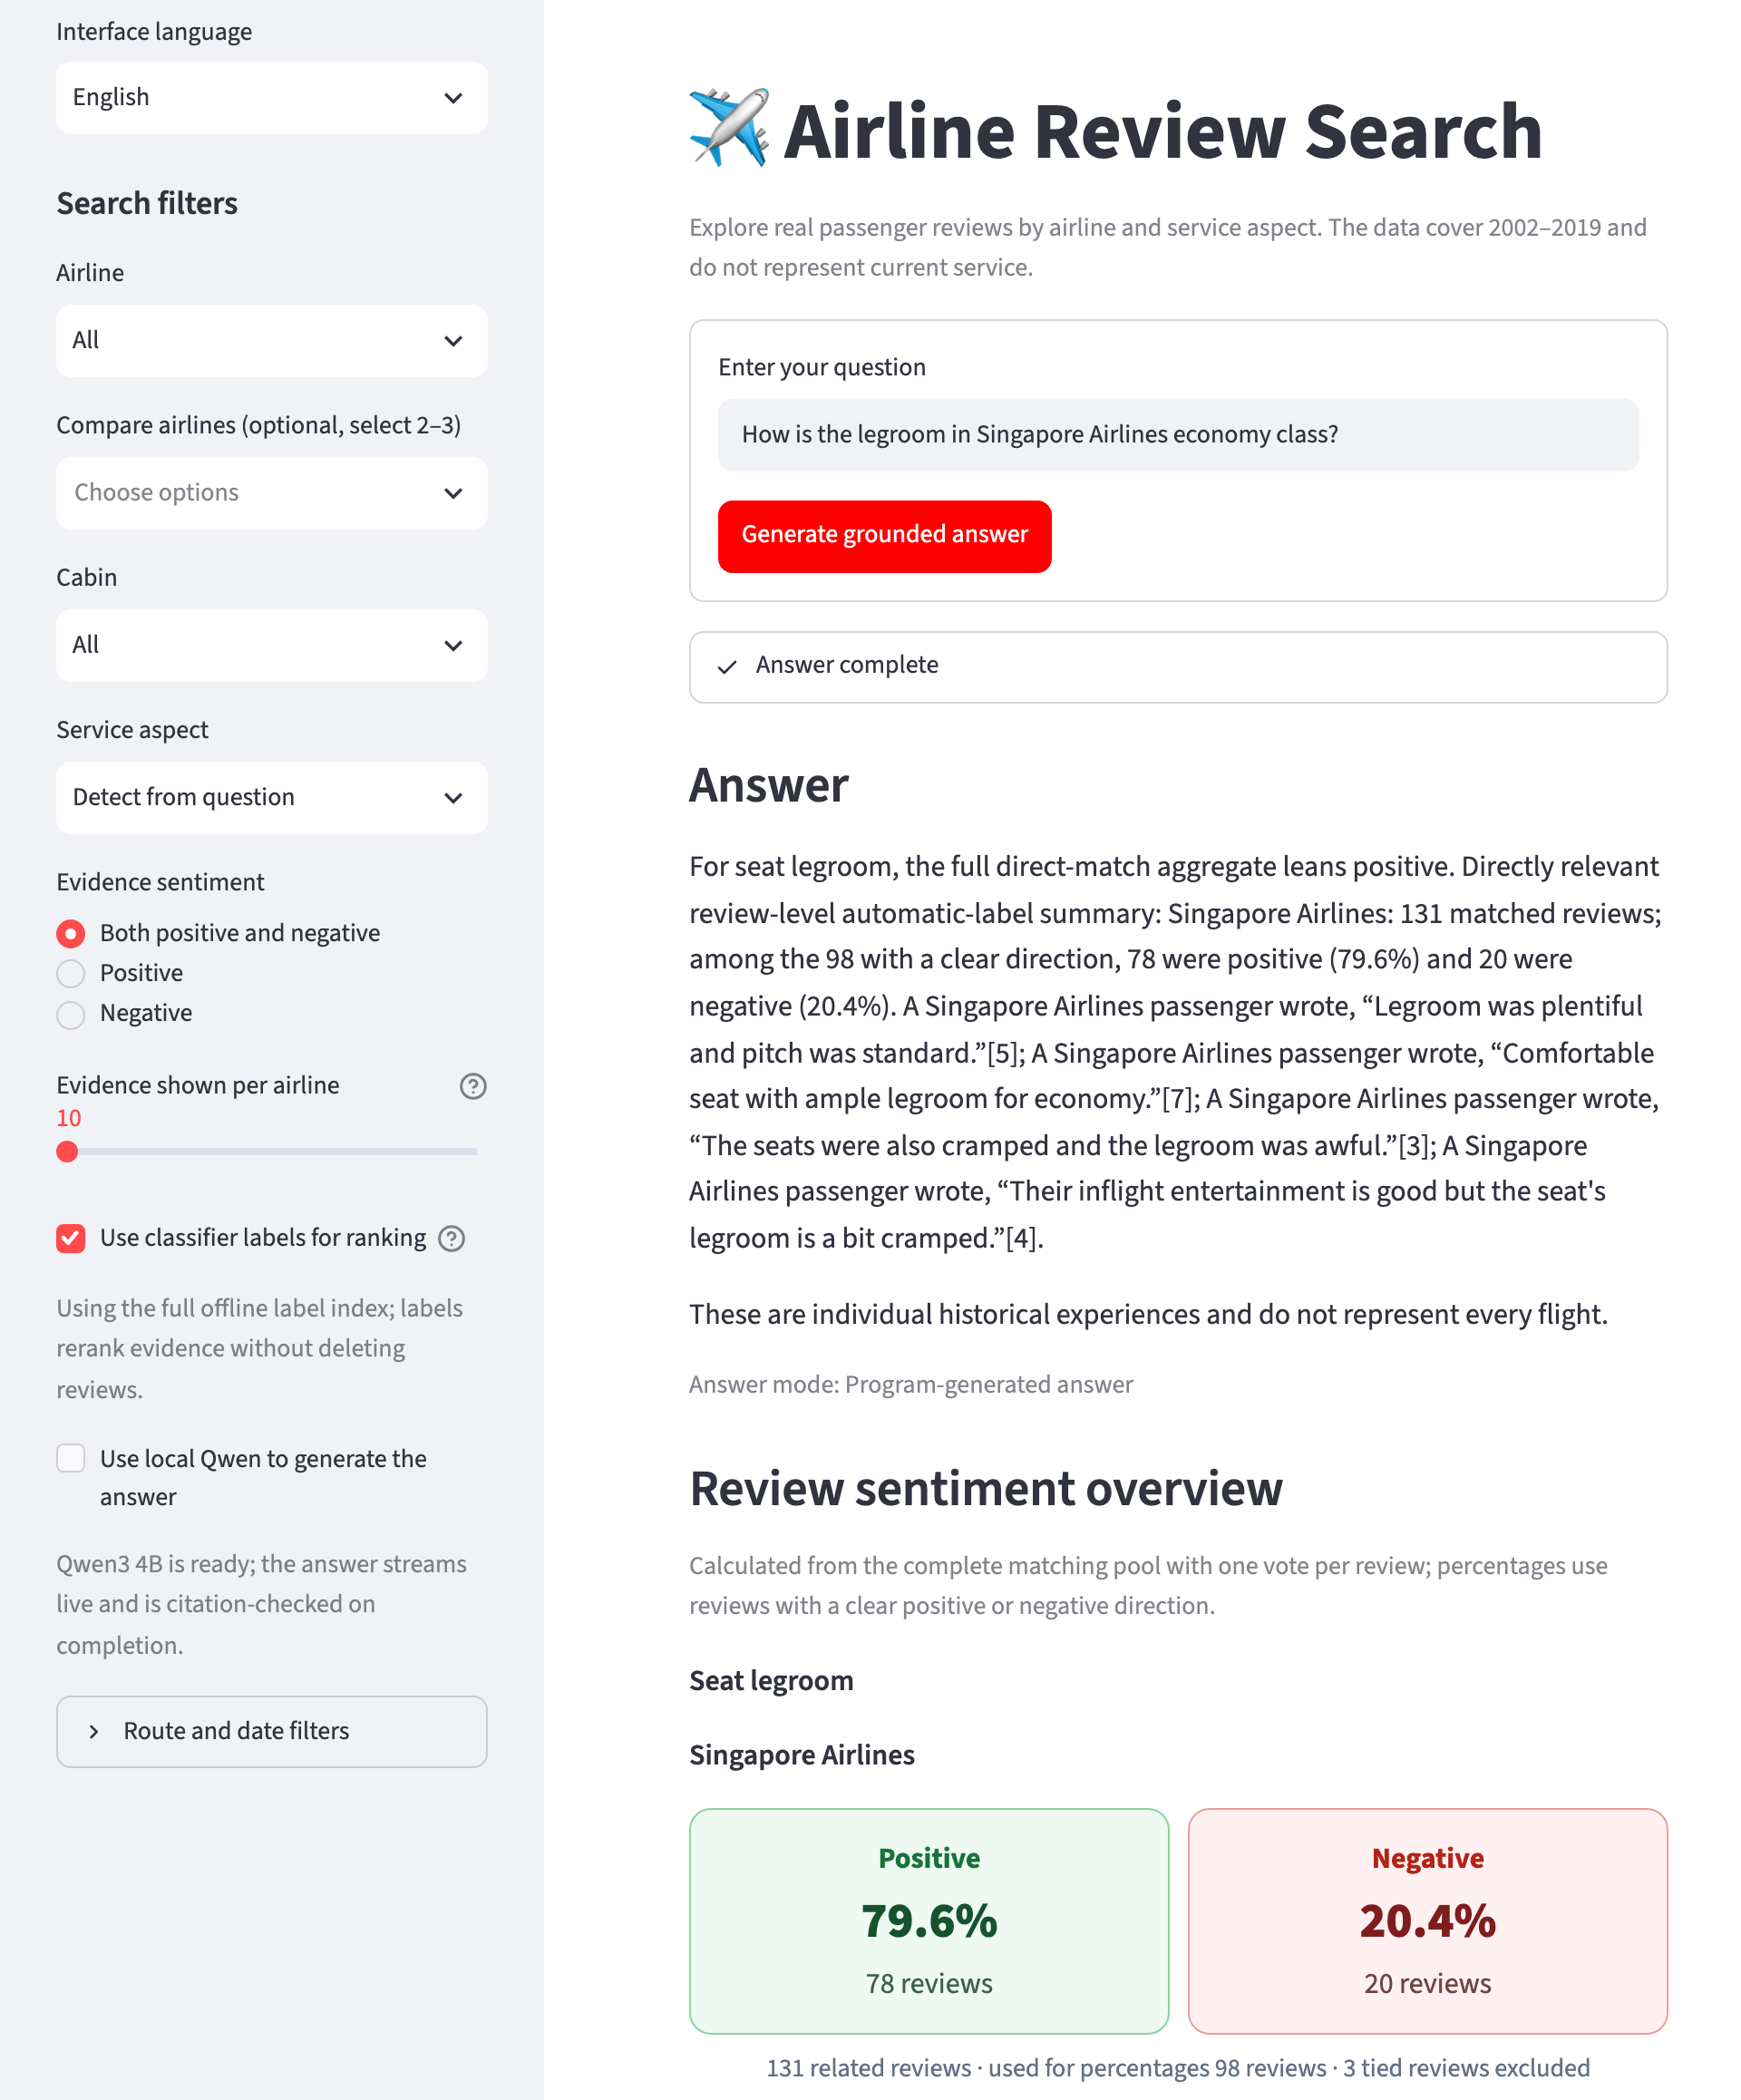
\includegraphics[width=\linewidth]{figures/ui_single.png}
\end{minipage}\hfill
\begin{minipage}[b]{0.33\textwidth}
\caption{界面：英文模式下的单航司问题。解析器识别出航司、方面（座椅）和细分属性（腿部空间）。程序生成的回答引用了四句话；概览统计了 131 条匹配评论，其中 98 条有明确倾向（79.6\% 正面）。侧栏是结构化过滤条件（航司、对比航司、舱位、方面、证据倾向，最后的折叠栏里是航线和日期）。}
\label{fig:ui}
\end{minipage}
\end{figure*}

\begin{figure*}[t]
\centering
\begin{subfigure}[t]{0.548\textwidth}
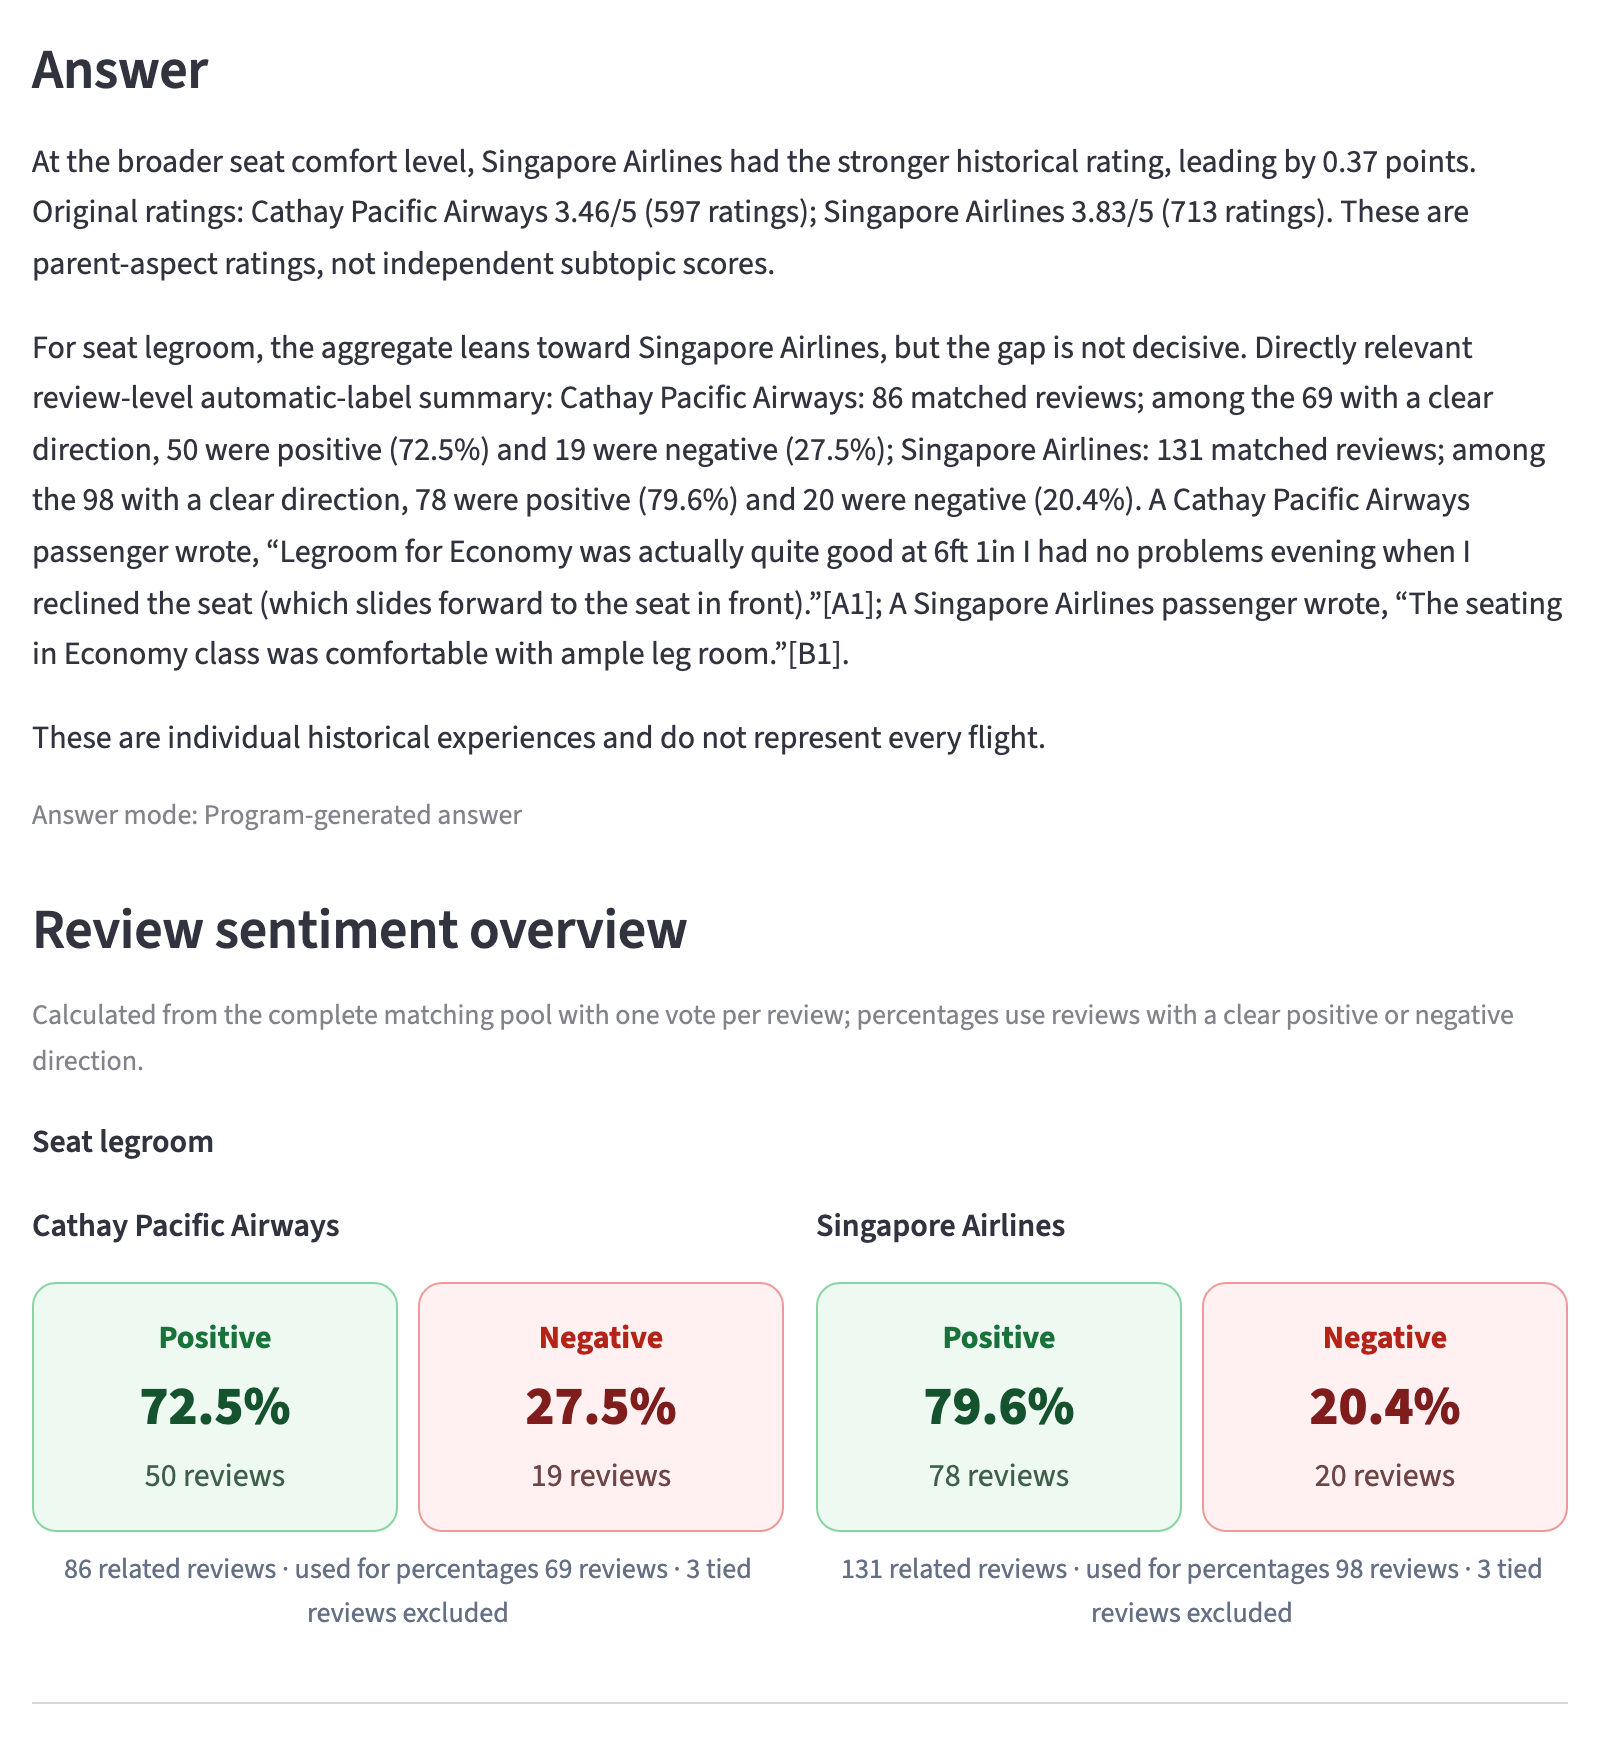
\includegraphics[width=\linewidth]{figures/ui_compare_answer.png}
\caption{回答（含评分检验）和全量统计。}
\end{subfigure}\hfill
\begin{subfigure}[t]{0.432\textwidth}
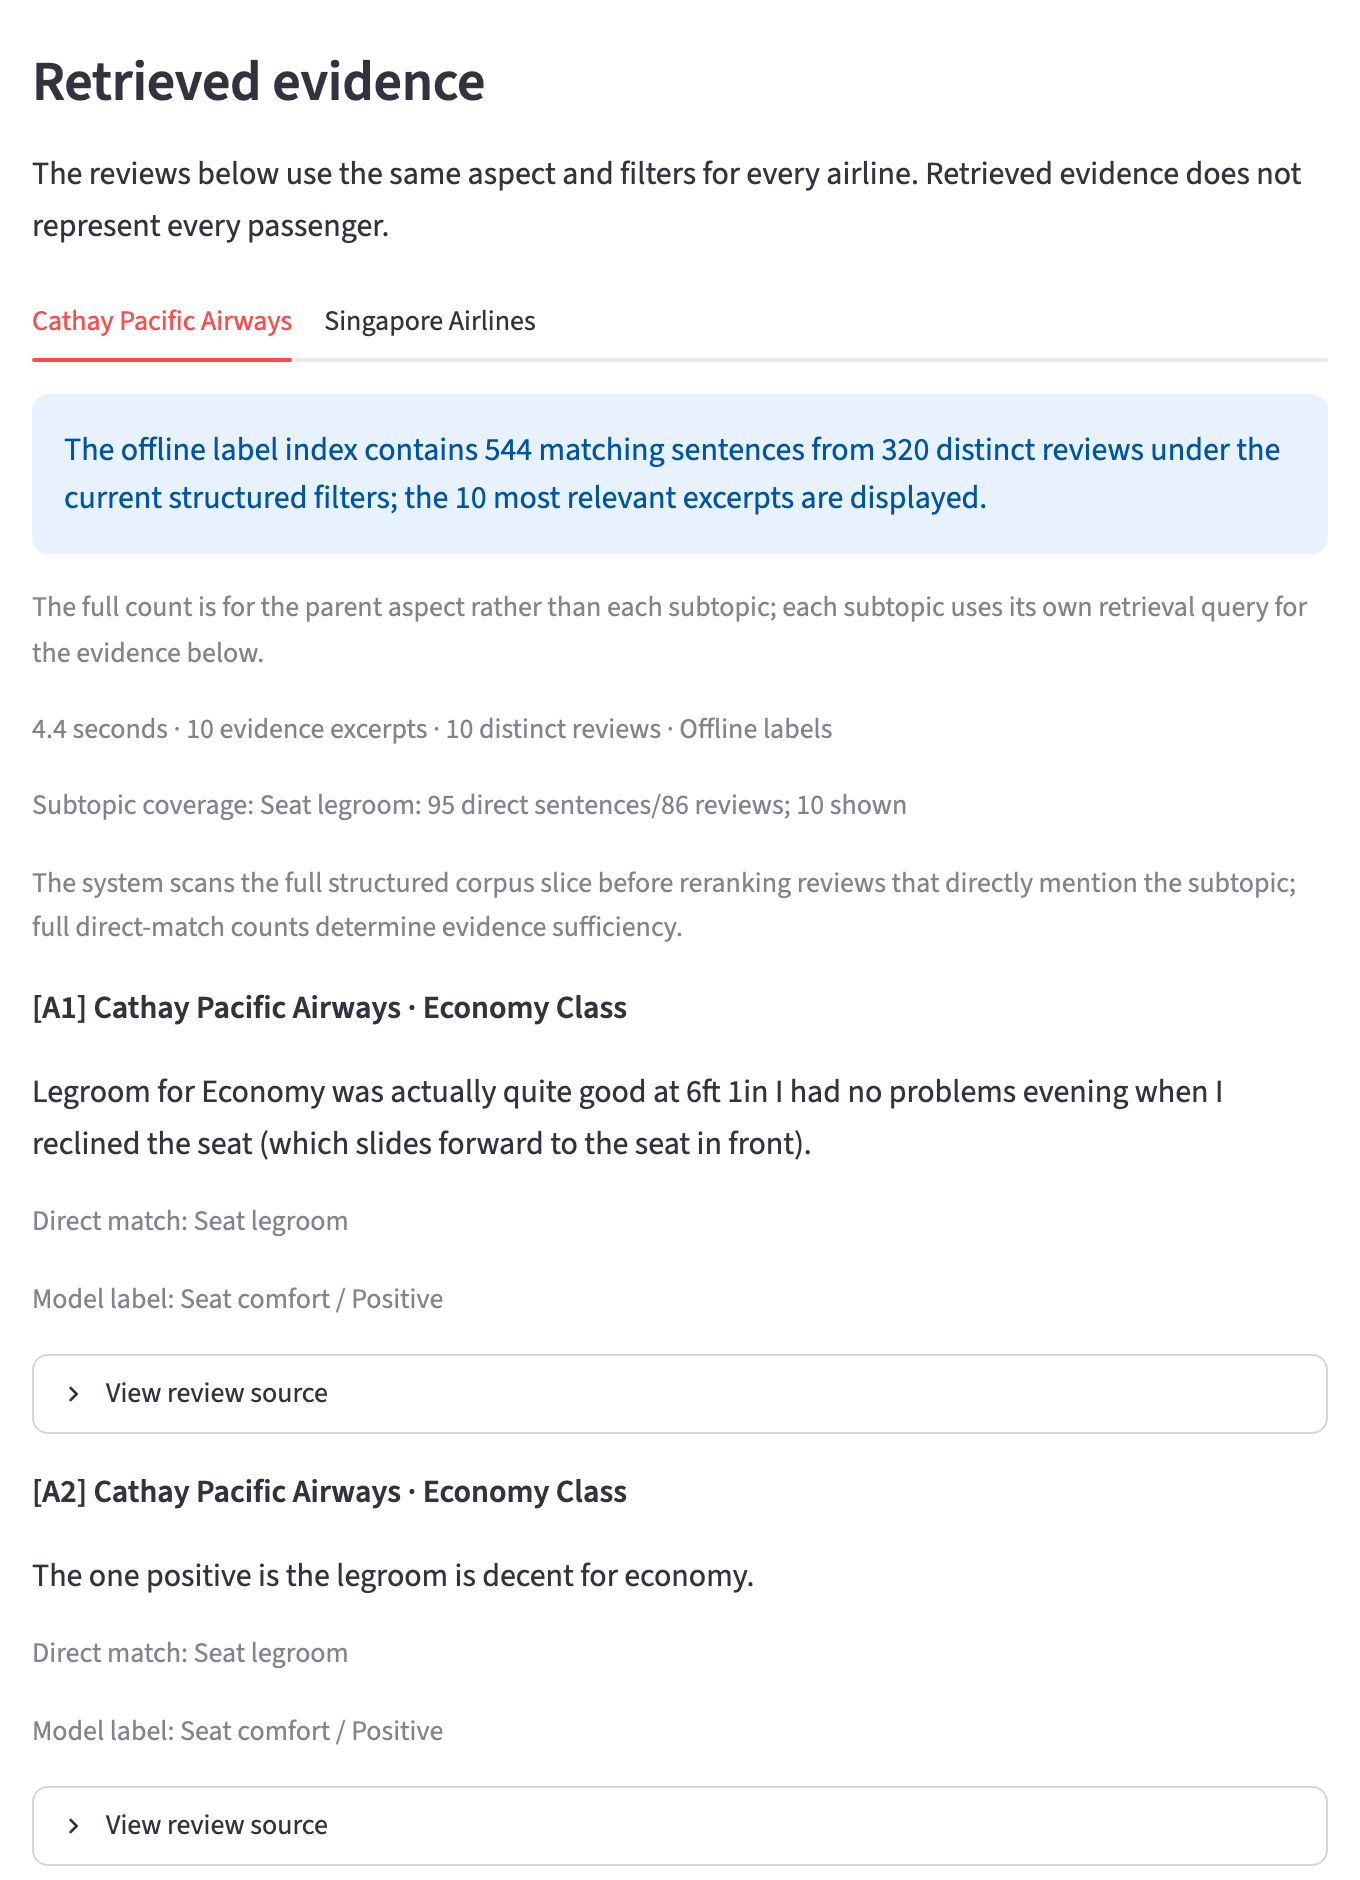
\includegraphics[width=\linewidth]{figures/ui_compare_evidence.png}
\caption{证据标签页及覆盖计数。}
\end{subfigure}
\caption{国泰航空与新加坡航空经济舱腿部空间对比。新加坡航空的座椅舒适度评分更高（3.83 对 3.46，满分 5），差距显著，作为上级方面的结论报告；腿部空间的统计（72.5\% 对 79.6\% 正面）报告为“差距不足以下结论”。证据页显示 86 条评论中有 95 句直接提到腿部空间，检索耗时 4.4\,s（与表~\ref{tab:five} 不是同一次运行）。}
\label{fig:ui-compare}
\end{figure*}

%--------------------------------------------------------------- 实验
\section{实验}
\label{sec:exp}

\subsection{实验设置与评估数据}
\label{sec:data}

全部实验都在 Apple M1 Pro（16\,GB）上运行。区间均为在查询、问题或所属评论层面重采样的 95\% bootstrap 区间（E1、E5 重采样 \num{10000} 次，E4、E6、E7 为 \num{2000} 次）。评估数据包括：30 个“航司 $\times$ 细分属性”检索单元（E1）；20 个用中文写的固定端到端问题（12 个单航司、5 个比较、3 个多方面；E2、E5）；\num{1000} 句人工标注的 gold 集（E3、E4）；析因消融用的 20 个英文单属性问题（E6，附录~\ref{app:factorial}）；以及航司排名所用的留出乘客评分（E7）。

\paragraph{Gold 集（Q4）。}候选来自去掉航线行、重复句、不足五个词的句子和无总评分评论后剩下的 \num{478969} 句。我们一半从总评分 $\ge$7 的评论中抽、一半从 $\le$4 的评论中抽，每个有评分的方面约 120 句，再加上没有明确方面的句子，然后打乱。三位标注者独立标注每一句，且\emph{只看得到句子本身}：航司和评分被隐藏，因为评分也是弱标签的来源。书面标注指南规定了混合情感等边界情况。在冻结的 \num{1000} 句上，三项任务的一致率都超过 80\%（表~\ref{tab:agree}）；主客观的 Fleiss' $\kappa$~\cite{fleiss} 只是中等，因为只有 8\% 的句子是客观句。在全部 \num{1100} 句标注上，作业要求的两项任务（主客观和极性）仍超过 80\%，但方面一致率为 75.2\%：被剔除的 100 句中，15 句是标注指南判为“看不清”的，52 句是三位标注者给了三个不同的方面。分歧先按多数投票解决，剩余的用 AI 辅助裁决，再由人工逐条确认，最终审核者改动了 9 句。抽样平衡了评论总评分（502 对 498 句），但没有平衡标签：高分评论里有 143 句是抱怨，而低分评论里只有 49 句是表扬。我们保留了这种自然偏斜，没有在标注后重新抽样，并报告宏平均和分类别指标。该集合有 548 句负面、371 句正面、81 句客观，无重复文本，以标准基准格式存为 \nolinkurl{data/eval/eval.xls}（附录~\ref{app:eval}）。

\begin{table}[t]
\centering\small
\caption{三位原始标注者的两两一致率。冻结集：\num{1000} 句 gold（\num{3000} 个标注者对），附 Fleiss' $\kappa$。全部：所有标注句子（\num{1100} 句，\num{3300} 对）。}
\label{tab:agree}
\setlength{\tabcolsep}{4pt}
\begin{tabular}{@{}lrrrr@{}}
\toprule
\textbf{字段} & \textbf{一致对数} & \textbf{冻结集} & \textbf{$\kappa$} & \textbf{全部} \\
\midrule
主客观 & \num{2783} & 92.8\% & 0.572 & 90.9\% \\
极性（含 NA） & \num{2730} & 91.0\% & 0.841 & 89.3\% \\
方面（8 类） & \num{2426} & 80.9\% & 0.778 & 75.2\% \\
三项同时一致 & \num{2250} & 75.0\% & 0.732 & 69.8\% \\
\bottomrule
\end{tabular}
\end{table}

\paragraph{Gold 集的适用范围。}我们共标注了 \num{1100} 句，冻结了其中 \num{1000} 句；这 1000 句是在标注\emph{之后}按“原始方面标签一致”挑出来的，因此冻结集上的一致率高于全部标注句子（表~\ref{tab:agree}）。开发过程中，一些早期分类器版本也在这些句子上评估过。所以我们把它当作一个仔细裁决过的基准，而不是一个从未接触过的测试集；对于蒸馏模型（E4），模型选择从未读取它，且只在它上面评估了一次。

\subsection{E1：混合检索的排序更好吗？（Q3）}
\label{sec:exp-ret}

\paragraph{实验设置。}30 个单元（如\emph{新加坡航空，腿部空间}）在各配置下使用相同的元数据约束。相关性自动分级：明确点名该细分属性的句子为高度相关；被分类器标为同一方面且为主观句的为部分相关。我们报告 P@5、Recall@50、MRR、NDCG@10~\cite{ndcg} 和 Success@10。

\begin{table*}[t]
\centering\small
\caption{E1：30 个“航司 $\times$ 细分属性”查询上的检索质量（自动分级相关性）。每列最优加粗；延迟为预热后每个查询的中位数，含元数据过滤。这些是检索器配置；线上流程还会在过滤后的子集里扫描细分属性的直接提及（\sref{sec:ret}）。}
\label{tab:retrieval}
\begin{tabular}{@{}lrrrrrr@{}}
\toprule
\textbf{配置} & \textbf{P@5} & \textbf{Recall@50} & \textbf{MRR} & \textbf{NDCG@10} & \textbf{Success@10} & \textbf{延迟} \\
\midrule
BM25 & \best{0.880} & \best{0.403} & 0.950 & 0.790 & 1.000 & 0.534\,s \\
稠密检索（MiniLM） & 0.753 & 0.307 & 0.867 & 0.686 & 1.000 & \best{0.057\,s} \\
\rowcolor{shade} 混合 + RRF（默认） & \best{0.880} & 0.381 & \best{0.961} & \best{0.810} & 1.000 & 0.592\,s \\
混合 + RRF + 交叉编码器 & 0.827 & 0.387 & 0.933 & 0.744 & 1.000 & 0.714\,s \\
\bottomrule
\end{tabular}
\end{table*}

\begin{figure}[t]
\centering
\begin{tikzpicture}
\begin{axis}[paper, barlegend, ybar, width=\columnwidth, height=44mm, bar width=6pt, ymin=0.6, ymax=1.0,
  symbolic x coords={P@5,MRR,NDCG@10}, xtick=data, enlarge x limits=0.25, ylabel={得分},
  legend style={at={(0.5,1.02)},anchor=south, legend columns=2}]
\addplot[fill=s1, draw=white] coordinates {(P@5,0.880) (MRR,0.950) (NDCG@10,0.790)};
\addplot[fill=s2, draw=white] coordinates {(P@5,0.753) (MRR,0.867) (NDCG@10,0.686)};
\addplot[fill=s3, draw=white] coordinates {(P@5,0.880) (MRR,0.961) (NDCG@10,0.810)};
\addplot[fill=s4, draw=white] coordinates {(P@5,0.827) (MRR,0.933) (NDCG@10,0.744)};
\legend{BM25, 稠密检索, 混合 + RRF, + 交叉编码器}
\end{axis}
\end{tikzpicture}
\caption{E1：表~\ref{tab:retrieval} 中偏重精确率的指标（纵轴从 0.6 开始）。}
\label{fig:retrieval}
\end{figure}

\paragraph{结果。}混合 + RRF 在 MRR 和 NDCG@10 上最好，P@5 与 BM25 持平（表~\ref{tab:retrieval}、图~\ref{fig:retrieval}）。单独的稠密检索最弱：它会把主题相关但属性不对的句子排得很靠前；融合保留了 BM25 的精确率，并在靠后位置补充同义改写。相对 BM25 的提升在 30 个查询下不显著（$\Delta$NDCG@10 $=+0.020$，区间 $[-0.036,+0.073]$）。交叉编码器反而\emph{有害}（$\Delta$NDCG@10 $=-0.066$，区间 $[-0.114,-0.019]$）：它在 MS MARCO 网页问答上训练，偏好“总体上回答了问题”的句子，例如一段很长的舒适度描述，而不是点名该属性的短句。因此我们只用它给已经提到所问细分属性的候选排序。各配置的 Success@10 都是 1.0，所以差异体现在排序和覆盖上。这些相关性标注可复现，但偏向明确提及，对 BM25 有利，并且低估了稠密检索找到的同义改写（如“膝盖顶到前排座椅”）；人工相关性判断会让比较更有说服力。

\paragraph{哪项创新最重要？（E1b）}E1 固定约束和查询、只改变检索器。为了衡量表~\ref{tab:fixes} 中各项创新本身的作用，我们从初版开始逐项重建这 30 个单元（表~\ref{tab:innov}）。这里的相关性不复用扩展词表：一条结果必须满足问题的约束（由元数据判断），并且本地 Qwen3-4B 在只看到属性英文名的情况下判断该句谈到了这个属性（是/否，共 620 次判断），才算相关。评判模型在 23 句人工编写的校准句上答对 22 句；随机抽查 40 次判断发现 6 处错误，多是把针对航司的泛泛抱怨判为相关，因此各行的绝对精确率都略偏乐观。

\begin{table*}[t]
\centering\small
\caption{E1b：在 E1 的 30 个单元上逐项加入表~\ref{tab:fixes} 的检索创新，均使用混合检索加 RRF。\emph{范围内}：前 10 条中满足问题的航司、舱位等约束的比例（由元数据精确判断）。P@5、MRR 和 NDCG@10（二值）只把既在范围内、又被 LLM 评判为“谈到该属性”的结果算作相关。\emph{直接}：前 10 条中明确点名该细分属性的比例（关键词匹配，与 R2 共用词表）。$\Delta$：相对上一行的 NDCG@10 变化及 95\% bootstrap 区间。}
\label{tab:innov}
\begin{tabular}{@{}lrrrrrl@{}}
\toprule
\textbf{配置} & \textbf{范围内} & \textbf{P@5} & \textbf{MRR} & \textbf{NDCG@10} & \textbf{直接} & \textbf{$\Delta$NDCG@10 [95\% CI]} \\
\midrule
初版：原样输入问题，检索全库 & 0.213 & 0.053 & 0.102 & 0.057 & 0.000 & \\
+ 解析为英文关键词（跨语言） & 0.350 & 0.160 & 0.389 & 0.173 & 0.070 & $+0.116$ [$+0.060$, $+0.175$] \\
+ R1 元数据硬约束 & \best{1.000} & 0.953 & \best{1.000} & 0.934 & 0.670 & $+0.761$ [$+0.673$, $+0.838$] \\
\rowcolor{shade} + R2 细分属性扩展（线上版本） & \best{1.000} & \best{0.967} & 0.983 & \best{0.951} & \best{0.837} & $+0.016$ [$-0.022$, $+0.057$] \\
\midrule
线上版本去掉 R1 & 0.160 & 0.127 & 0.297 & 0.121 & 0.097 & $-0.830$ [$-0.892$, $-0.763$] \\
\bottomrule
\end{tabular}
\end{table*}

硬约束带来的提升远大于其他各项。没有硬约束时，前 10 条中只有 16--35\% 来自所问的航司和舱位，因为谈腿部空间的那句话很少点名航司；加上之后每条结果都满足约束，NDCG@10 提高 0.761。把中文问题解析为英文关键词使 NDCG@10 从 0.057 升到 0.173，因为 BM25 和英文 MiniLM 都无法用中文去匹配英文语料。有了约束之后，细分属性扩展的提升很小（$+0.016$，不显著）：在单一航司和舱位的子集里，仅用属性名就已能找到切题的句子。它提高的是明确点名该细分属性的结果比例（0.67 升到 0.84），而全子集扫描（R3）依赖的正是这类句子。R3 本身不需要排序指标来衡量：即使是最好的配置，前 50 条也只覆盖 38\% 的直接提及句（表~\ref{tab:retrieval} 的 Recall@50），所以只按前 $k$ 条得出的结论只看到了少数证据。

\subsection{E2：一次查询有多快？（Q2）}
\label{sec:exp-speed}

表~\ref{tab:five} 报告了 20 个评估问题中的 5 个，它们覆盖了系统支持的各类查询，均为开启本地模型、预热后的运行结果。\emph{检索}包括解析、过滤、BM25、稠密检索、融合、重排和证据挑选；\emph{首字}从提交开始计时；\emph{总计}截止到展示通过校验的回答。图~\ref{fig:latency} 显示检索只占等待时间的一小部分，主要耗时来自笔记本上的 4B 模型，我们用流式输出来缓解。不加过滤、在完整检索池上单独计时（E1 的 30 个查询，预热后中位数）：BM25 top-20 为 503\,ms，FAISS top-20 为 20\,ms，混合检索（两路 top-100 加 RRF）为 519\,ms，交叉编码器重排 100 个候选为 108\,ms（\nolinkurl{experiments/final_auto_eval/component_latency.py}）；主要耗时是 BM25 给全部句子打分。关闭 LLM 时，程序生成回答在 40 个问题的冒烟测试中平均每题 5.0\,s。

\begin{table}[t]
\centering\small
\caption{E2：五个代表性查询（中文提问，原文和结果见附录~\ref{app:queries}）。回答来源：模型草稿（D）、修复稿（R）或程序生成（P）。“全部 20 题”两行包含冷启动的第一题。}
\label{tab:five}
\setlength{\tabcolsep}{3.5pt}
\begin{tabularx}{\columnwidth}{@{}lYrrrc@{}}
\toprule
& \textbf{查询} & \textbf{检索} & \textbf{首字} & \textbf{总计} & \textbf{来源} \\
\midrule
Q05 & 阿联酋经济舱：退款和改签？ & 2.2\,s & 23.8\,s & 26.8\,s & D \\
Q10 & 卡塔尔商务舱：电影选择？ & 2.2\,s & 18.4\,s & 33.6\,s & R \\
Q24 & 国泰 vs.\ 新航经济舱腿部空间？ & 5.1\,s & 28.4\,s & 57.8\,s & R \\
Q28 & 新航经济舱：腿部空间、靠背、舒适度、清洁度？ & 9.7\,s & 27.4\,s & 53.6\,s & P \\
Q30 & 新航经济舱：餐食、性价比、地面服务？ & 6.9\,s & 50.8\,s & 82.0\,s & P \\
\midrule
\multicolumn{2}{@{}l}{\textit{全部 20 题：中位数}} & 2.9\,s & 24.3\,s & 40.8\,s & \\
\multicolumn{2}{@{}l}{\textit{全部 20 题：P95}} & 10.5\,s & 41.9\,s & 72.3\,s & \\
\bottomrule
\end{tabularx}
\end{table}

\begin{figure}[t]
\centering
\begin{tikzpicture}
\begin{axis}[paper, xbar stacked, width=\columnwidth, height=40mm, barlegend, bar width=7pt,
  xmin=0, xmax=85, xlabel={秒}, ymajorgrids=false, xmajorgrids,
  symbolic y coords={Q30,Q28,Q24,Q10,Q05}, ytick=data, y dir=reverse,
  legend style={at={(0.5,1.03)},anchor=south, legend columns=3}, enlarge y limits=0.15]
\addplot[fill=s1, draw=white] coordinates {(2.2,Q05) (2.2,Q10) (5.1,Q24) (9.7,Q28) (6.9,Q30)};
\addplot[fill=s2, draw=white] coordinates {(21.6,Q05) (16.2,Q10) (23.3,Q24) (17.7,Q28) (43.9,Q30)};
\addplot[fill=s3, draw=white] coordinates {(3.0,Q05) (15.2,Q10) (29.4,Q24) (26.2,Q28) (31.2,Q30)};
\legend{检索, 等待首字, 生成 + 校验 + 修复}
\end{axis}
\end{tikzpicture}
\caption{E2：表~\ref{tab:five} 中各查询的耗时构成。}
\label{fig:latency}
\end{figure}

\subsection{E3：分类器效果如何？（Q4）}
\label{sec:exp-cls}

表~\ref{tab:cls} 给出用于模型选择的汇总指标（919 个主观句上方面和极性的宏 F1、联合准确率、主客观各类召回率）；表~\ref{tab:prf} 按作业要求给出各类的精确率、召回率和 F1；图~\ref{fig:aspect} 给出各方面的 F1。

\begin{table}[t]
\centering\small
\caption{E3：gold 集上的分类器质量（\%）。方面和极性 F1 为 919 个主观句上的宏平均。灰底：选出、将替换 v4.1 的蒸馏学生模型（\sref{sec:exp-distill}）。联合：方面和极性都正确；S-rec./O-rec.：全部 \num{1000} 句上主观/客观句的召回率。v4.1 是界面当前使用的弱监督分类器；r36 是 LLM 教师（表~\ref{tab:approach}）；目标在项目开始时设定。}
\label{tab:cls}
\setlength{\tabcolsep}{3pt}
\begin{tabularx}{\columnwidth}{@{}Yrrrrr@{}}
\toprule
\textbf{模型} & \textbf{方面} & \textbf{极性} & \textbf{联合} & \textbf{主观召回} & \textbf{客观召回} \\
\midrule
v4.1：TF-IDF + 规则（弱标签） & 61.1 & 82.1 & 56.1 & 99.9 & 7.4 \\
TF-IDF + MiniLM（弱标签） & 68.1 & 85.2 & 61.5 & \best{100.0} & 21.0 \\
\rowcolor{shade} 蒸馏模型（弱 + 教师） & 70.4 & 86.2 & 63.5 & 96.8 & 66.7 \\
r36 LLM 教师 & \best{74.1} & \best{91.8} & \best{70.8} & 96.8 & \best{76.5} \\
\midrule
\textit{项目目标} & 85 & 90 & 80 & 97 & -- \\
\bottomrule
\end{tabularx}
\end{table}

\begin{table*}[t]
\centering\small
\caption{E3：各类精确率 / 召回率 / F1（\%）。三分类标签即 eval.xls 的 \texttt{label} 列。极性在 919 个 gold 主观句上计算，被错判为“客观”的句子计为漏判。}
\label{tab:prf}
\begin{tabular}{@{}l*{3}{rrr}@{}}
\toprule
 & \multicolumn{3}{c}{\textbf{v4.1（原版）}} & \multicolumn{3}{c}{\textbf{蒸馏学生模型}} & \multicolumn{3}{c}{\textbf{r36 教师}} \\
\cmidrule(lr){2-4}\cmidrule(lr){5-7}\cmidrule(l){8-10}
\textbf{类别} & P & R & F1 & P & R & F1 & P & R & F1 \\
\midrule
\multicolumn{10}{@{}l}{\textit{三分类标签}} \\
\quad 负面 & 76.8 & 88.3 & 82.2 & 87.9 & 87.4 & 87.6 & 91.4 & 93.4 & 92.4 \\
\quad 正面 & 76.6 & 74.9 & 75.7 & 82.0 & 82.2 & 82.1 & 92.0 & 86.5 & 89.2 \\
\quad 客观 & 85.7 & 7.4 & 13.6 & 65.1 & 66.7 & 65.9 & 68.1 & 76.5 & 72.1 \\
\quad 宏平均 & 79.7 & 56.9 & 57.2 & 78.3 & 78.8 & \best{78.5} & 83.8 & 85.5 & 84.6 \\
\quad 准确率 & \multicolumn{3}{r}{76.8} & \multicolumn{3}{r}{\best{83.8}} & \multicolumn{3}{r}{89.5} \\
\midrule
\multicolumn{10}{@{}l}{\textit{主客观判断}} \\
\quad 主观 & 92.4 & 99.9 & 96.0 & 97.1 & 96.8 & 96.9 & 97.9 & 96.8 & 97.4 \\
\quad 客观 & 85.7 & 7.4 & 13.6 & 65.1 & 66.7 & 65.9 & 68.1 & 76.5 & 72.1 \\
\midrule
\multicolumn{10}{@{}l}{\textit{极性判断（gold 主观句）}} \\
\quad 负面 & 83.9 & 88.3 & 86.0 & 89.9 & 87.4 & 88.6 & 93.3 & 93.4 & 93.3 \\
\quad 正面 & 81.5 & 74.9 & 78.1 & 85.4 & 82.2 & 83.8 & 94.1 & 86.5 & 90.2 \\
\bottomrule
\end{tabular}
\end{table*}

\begin{figure}[t]
\centering
\begin{tikzpicture}
\begin{axis}[paper, ybar, width=\columnwidth, height=46mm, barlegend, bar width=3.6pt, ymin=0, ymax=100,
  symbolic x coords={娱乐,餐食,地面,座椅,性价比,员工,总体,其他},
  xtick=data, enlarge x limits=0.07, ylabel={F1（\%）}, legend style={at={(0.5,1.02)},anchor=south}]
\addplot[fill=s1, draw=white, line width=0.3pt] coordinates {(娱乐,83.1) (餐食,73.7) (地面,74.3) (座椅,77.9) (性价比,67.8) (员工,55.7) (总体,32.9) (其他,23.4)};
\addplot[fill=s2, draw=white, line width=0.3pt] coordinates {(娱乐,86.9) (餐食,79.3) (地面,82.8) (座椅,81.7) (性价比,75.6) (员工,64.8) (总体,57.4) (其他,35.0)};
\addplot[fill=s3, draw=white, line width=0.3pt] coordinates {(娱乐,87.3) (餐食,88.2) (地面,84.2) (座椅,88.6) (性价比,76.3) (员工,68.6) (总体,64.3) (其他,35.7)};
\legend{v4.1, 蒸馏模型, r36 教师}
\end{axis}
\end{tikzpicture}
\caption{E3：gold 主观句上各方面的 F1（样本数：娱乐 115、餐食 99、地面 238、座椅 86、性价比 130、员工 103、总体 101、其他 47）。具体方面容易；\emph{总体}和\emph{其他}对所有模型都难。}
\label{fig:aspect}
\end{figure}

\paragraph{结果。}客观句是弱监督的主要短板：只有 179 个客观训练样例，v4.1 只找出 7.4\% 的客观句，嵌入模型找出 21.0\%；加入教师标签后提高到 66.7\%，代价是主观召回下降 3 个点，三分类宏 F1 从 57.2 升到 78.5。方面错误集中在少数几类：学生模型最常见的混淆是\emph{员工}被判成\emph{餐食}（18 句，大多是空乘如何提供餐饮服务，例如 “No refills of drinks offered during or after the meal”）、\emph{地面}被判成\emph{性价比}（16 句，大多关于退款和赔偿），以及\emph{总体}与\emph{其他}互混。这些句子确实同时涉及两个方面，所以与 85\% 目标的差距有一部分来自“每句只标一个方面”的定义。没有任何模型（包括 LLM 教师）达到全部目标；我们如实报告，而不是在 gold 集上调参。

\subsection{E4：快速分类器能学到 LLM 的标注吗？（Q5）}
\label{sec:exp-distill}

\paragraph{动机。}标签索引决定了用户看到的统计。用 v4.1 构建时，语料中只有 0.6\% 被标为客观，而 gold 集中是 8.1\%，因此几乎所有事实陈述句都被当作观点计数。教师模型好得多，但标完全语料约需三天。

\paragraph{实验流程。}(i)~从弱标签\emph{开发集}的 \num{1154} 条评论中抽取 \num{10003} 句，排除所有 gold 句、其所属评论和规范化文本，以及弱标签训练中出现过的文本。(ii)~教师用 89 分钟标完全部句子，无无效输出（12.8\% 为客观）。(iii)~按所属评论划分为伪训练集（\num{7355}）和伪开发集（\num{2648}）。(iv)~训练前就固定三个特征相同、只有监督来源不同的学生模型：\emph{weak}（只用弱标签，复现一位组员的模型）、\emph{teacher}（只用教师标签）、\emph{mixed}（两者都用，教师样本加权使两种来源总权重相等）。(v)~用一个固定的排名分数（$0.35\,$方面 F1 $+\,0.20\,$极性 F1 $+\,0.35\,$联合准确率 $+\,0.10\,$主观召回，主观召回低于 97\% 或客观召回低于 60\% 时扣分），在伪开发集上以\emph{教师}为参照选出胜者；文件读取保护确保无法访问 gold。(vi)~同样事先规定：胜者只有在 gold 上的排名分数和联合准确率都超过 v4.1 时，才替换 v4.1。

\begin{table*}[t]
\centering\small
\caption{E4：监督来源消融。左：在伪开发集上与教师的一致程度（用于模型选择）。右：同一批模型在人工 gold 上的结果，选择完成后只评估一次。特征完全相同，只有训练标签不同。}
\label{tab:distill}
\begin{tabular}{@{}lrrr@{\hspace{8mm}}rrrr@{}}
\toprule
 & \multicolumn{3}{c}{\textbf{对照教师，伪开发集}} & \multicolumn{4}{c}{\textbf{对照人工 gold}} \\
\cmidrule(r{8mm}){2-4}\cmidrule(l){5-8}
\textbf{监督来源} & \textbf{联合} & \textbf{客观召回} & \textbf{排名分} & \textbf{方面 F1} & \textbf{联合} & \textbf{客观召回} & \textbf{排名分} \\
\midrule
v4.1 线上版本（参照） & 54.0 & 3.9 & 0.637 & 61.1 & 56.1 & 7.4 & 0.648 \\
只用弱标签 & 59.9 & 18.9 & 0.692 & 68.1 & 61.5 & 21.0 & 0.705 \\
只用教师标签（7.4k） & 64.0 & \best{75.7} & 0.662 & \best{71.4} & 61.4 & \best{76.5} & 0.651 \\
\rowcolor{shade} 弱 + 教师（入选） & \best{65.8} & 67.1 & \best{0.729} & 70.4 & \best{63.5} & 66.7 & \best{0.735} \\
\bottomrule
\end{tabular}
\end{table*}

\begin{figure}[t]
\centering
\begin{tikzpicture}
\begin{axis}[paper, width=0.74\columnwidth, height=46mm,
  xmin=-12, xmax=12, ymin=0.4, ymax=4.6, ytick={1,2,3,4}, y dir=reverse,
  yticklabels={入选 vs v4.1, 弱标签 vs v4.1, 入选 vs 弱标签, 入选 vs r36},
  ymajorgrids=false, xmajorgrids, xlabel={联合准确率差值（百分点，95\% 区间）},
  extra x ticks={0}, extra x tick labels={}, extra x tick style={grid style={draw=black, line width=0.6pt}}]
\addplot[only marks, mark=*, mark size=2.2pt, color=s1, mark options={draw=white},
  error bars/.cd, x dir=both, x explicit, error bar style={draw=s1, line width=1.1pt}, error mark options={draw=s1, line width=1.1pt, mark size=2.2pt, rotate=90}]
  coordinates {(7.4,1) -= (2.9,0) += (3.0,0)  (5.3,2) -= (2.7,0) += (2.8,0)  (2.1,3) -= (2.2,0) += (2.2,0)  (-7.3,4) -= (3.1,0) += (3.2,0)};
\node[font=\sffamily\tiny, anchor=south] at (axis cs:7.4,1) [yshift=3.5pt] {+7.4};
\node[font=\sffamily\tiny, anchor=south] at (axis cs:5.3,2) [yshift=3.5pt] {+5.3};
\node[font=\sffamily\tiny, anchor=south] at (axis cs:2.1,3) [yshift=3.5pt] {+2.1};
\node[font=\sffamily\tiny, anchor=south] at (axis cs:-7.3,4) [yshift=3.5pt] {$-$7.3};
\end{axis}
\end{tikzpicture}
\caption{E4：gold 上联合准确率的配对差值（按所属评论 bootstrap）。区间依次为 $[+4.5,+10.4]$、$[+2.6,+8.1]$、$[-0.1,+4.3]$、$[-10.4,-4.1]$。}
\label{fig:distill}
\end{figure}

\paragraph{结果。}mixed 学生模型在伪开发集上入选，并在 gold 上通过了采用规则（表~\ref{tab:distill}）。把 v4.1 的特征换成 TF-IDF + MiniLM 带来 +5.3 个点的联合准确率（与 v4.1 的规则层混杂）；再加入教师标签又带来 +2.1，在 95\% 水平上不显著（区间 $[-0.1,+4.3]$，图~\ref{fig:distill}），并把客观召回从 21.0\% 提高到 66.7\%。教师标签的单位价值很高：只用 7.4k 句教师标签训练的学生，方面 F1 和客观召回是三者中最好的，但极性不如同时用了 \num{231779} 条弱标签的模型，所以两者混合总体最好。重建 \num{529031} 条标签的索引只需 18\,s，而教师估计需要三天；语料中客观句占比从 0.6\% 变为 13.0\%（教师在样本上为 12.8\%），32\% 的方面标签和 24\% 的极性标签发生变化。学生模型仍比教师低 7.3 个点。

\paragraph{现状。}由于三分之一的标签发生了变化，界面要等下游统计重新跑完后才切换到新索引；下文 E5 和 E6 用的是 v4.1 标签，E7 用的是另一个专门的诊断分类器（TF-IDF 加逻辑回归）。

\subsection{E5：回答是否有据可依？（Q4）}
\label{sec:exp-rag}

我们在 20 个问题上用 RAGAS 风格的指标~\cite{ragas} 评估整个系统：\emph{忠实度}（回答中有证据支持的论断占比）、\emph{答案相关性}、\emph{上下文精确率}（展示的证据中与问题相关的占比）。评判者是本地 Qwen3-4B，使用固定评分标准；它能看到展示的证据和程序算出的评分与统计，这样正确的汇总数字不会被判为无依据。

\begin{table}[t]
\centering\small
\caption{E5：带校验系统的回答级指标（20 个问题）。}
\label{tab:rag}
\begin{tabular}{@{}lrl@{}}
\toprule
\textbf{指标} & \textbf{得分} & \textbf{95\% 区间} \\
\midrule
忠实度 & 0.843 & [0.800, 0.890] \\
答案相关性 & 0.988 & [0.963, 1.000] \\
上下文精确率 & 0.600 & [0.517, 0.681] \\
\bottomrule
\end{tabular}
\end{table}

\paragraph{结果。}回答切题，且大多有据（表~\ref{tab:rag}）。上下文精确率最弱：约 40\% 的展示句被判为与问题不直接相关，部分原因是我们刻意展示反例和上级方面的背景（E6）。这些分数描述的是\emph{整个系统}：1 个问题用的是模型初稿，3 个用的是修复稿，16 个用的是程序生成的回答，因为 4B 模型的草稿经常过不了严格的引用或数字校验。由于生成器和评判者是同一个模型，这些是可复现的自动代理指标，而不是独立的人工评分。

\subsection{E6：每个回答端组件带来了什么？（Q5）}
\label{sec:exp-abl}

作业要求给出每项创新单独加入以及组合加入时的收益。因此我们对\sref{sec:gen}的三个因素做了完整的 $2^3$ 析因消融：X（全量统计）、Y（正反平衡且与标签一致的示例）、Z（校验、一次修复、程序后备）。

\paragraph{实验设置。}使用开发冒烟集中的 20 个单航司、单属性问题 Q01--Q20，改写成固定的英文句式（附录~\ref{app:factorial}），在评分前固定。每题有一个 30 条候选的冻结候选池，排序不借助标签；八种配置共享候选池、提示词和最多四条引用的预算。X 关闭时，全量统计和总体倾向对生成、校验和后备都不可见（提示词中引用它们的那条规则换成“描述展示出的证据”）；Y 关闭时，使用排序前四条候选；Z 关闭时，直接返回未经检查的模型初稿。线上使用的 Qwen3-4B-Instruct-2507（4-bit，MLX）同时负责生成和评判，评判沿用 E5 的评判器，且每种配置给评判者的程序统计相同。每题在每种 X/Y 设置下生成一份初稿，由 Z 关闭和开启两个版本共用，因此整个实验产生 80 份初稿、64 次修复尝试和 160 条最终回答（其中 144 条互不相同，各评判一次）。区间来自以题目为单位的 2,000 次配对 bootstrap（随机种子 6127），未做多重比较校正。

\begin{table*}[t]
\centering\small
\caption{E6：析因消融（每种配置 20 题）。编码依次为 XYZ，1 表示开启。$\Delta$：忠实度相对基线的配对差值及 95\% bootstrap 区间。160 条回答的答案相关性全部为 1.000。}
\label{tab:factorial}
\begin{tabular}{@{}llrlrr@{}}
\toprule
\textbf{编码} & \textbf{配置} & \textbf{忠实度} & \textbf{相对基线 $\Delta$ [95\% 区间]} & \textbf{上下文精确率} & \textbf{引用数} \\
\midrule
000 & 基线 & 0.890 & -- & 0.963 & 3.35 \\
100 & 仅 X & 0.841 & $-0.049$ [$-0.103$, $+0.007$] & 0.913 & 3.25 \\
010 & 仅 Y & 0.874 & $-0.016$ [$-0.079$, $+0.046$] & 0.925 & 3.45 \\
\rowcolor{shade} 001 & 仅 Z & \best{0.970} & $+0.080$ [$+0.041$, $+0.123$] & \best{0.988} & 3.90 \\
110 & X + Y & 0.846 & $-0.045$ [$-0.097$, $+0.011$] & 0.925 & 3.10 \\
101 & X + Z & 0.869 & $-0.022$ [$-0.077$, $+0.034$] & 0.813 & 3.10 \\
011 & Y + Z & 0.943 & $+0.053$ [$-0.012$, $+0.112$] & 0.950 & 3.50 \\
111 & X + Y + Z（线上配置） & 0.869 & $-0.022$ [$-0.070$, $+0.027$] & 0.938 & 3.55 \\
\bottomrule
\end{tabular}
\end{table*}

\begin{figure}[t]
\centering
\begin{tikzpicture}
\begin{axis}[paper, width=0.74\columnwidth, height=50mm,
  xmin=-0.12, xmax=0.14, ymin=0.4, ymax=7.6, ytick={1,2,3,4,5,6,7}, y dir=reverse,
  yticklabels={仅 X, 仅 Y, 仅 Z, X + Y, X + Z, Y + Z, X + Y + Z},
  ymajorgrids=false, xmajorgrids, xlabel={相对基线的忠实度 $\Delta$（95\% 区间）},
  xtick={-0.1,-0.05,0,0.05,0.1}, scaled x ticks=false,
  xticklabel={\pgfmathprintnumber[assume math mode=true,fixed,precision=2]{\tick}},
  extra x ticks={0}, extra x tick labels={}, extra x tick style={grid style={draw=black, line width=0.6pt}}]
\addplot[only marks, mark=*, mark size=2.2pt, color=s1, mark options={draw=white},
  error bars/.cd, x dir=both, x explicit, error bar style={draw=s1, line width=1.1pt}, error mark options={draw=s1, line width=1.1pt, mark size=2.2pt, rotate=90}]
  coordinates {(-0.0489,1) -= (0.0543,0) += (0.0560,0)  (-0.0163,2) -= (0.0628,0) += (0.0618,0)  (0.0796,3) -= (0.0385,0) += (0.0433,0)
               (-0.0446,4) -= (0.0526,0) += (0.0557,0)  (-0.0218,5) -= (0.0553,0) += (0.0554,0)  (0.0530,6) -= (0.0651,0) += (0.0588,0)
               (-0.0218,7) -= (0.0479,0) += (0.0490,0)};
\end{axis}
\end{tikzpicture}
\caption{E6：各配置相对基线的忠实度（数据见表~\ref{tab:factorial}）。只有“仅 Z”的区间完全在零以上。}
\label{fig:factorial}
\end{figure}

\begin{table}[t]
\centering\small
\caption{E6：主效应与交互效应（20 道配对题）。主效应为组件开启减关闭的差值，在另外两个因素的四种设置上取平均；XY 为 Y 开与关时 X 效应之差（对 Z 取平均），XYZ 为 Z 开与关时 XY 交互之差。上下文精确率是评判者看着回答打的分，所以即使展示的证据相同也会变动。}
\label{tab:effects}
\begin{tabular}{@{}lrlr@{}}
\toprule
\textbf{效应} & \multicolumn{2}{c}{\textbf{忠实度 [95\% 区间]}} & \textbf{上下文精确率} \\
\midrule
X & $-0.063$ & [$-0.099$, $-0.026$] & $-0.059$ \\
Y & $-0.010$ & [$-0.040$, $+0.017$] & $+0.016$ \\
Z & $+0.050$ & [$+0.027$, $+0.073$] & $-0.009$ \\
XY & $+0.024$ & [$-0.029$, $+0.078$] & $+0.106$ \\
XZ & $-0.050$ & [$-0.112$, $+0.012$] & $-0.069$ \\
YZ & $-0.007$ & [$-0.056$, $+0.044$] & $+0.056$ \\
XYZ & $+0.006$ & [$-0.069$, $+0.076$] & $+0.113$ \\
\bottomrule
\end{tabular}
\end{table}

\paragraph{结果。}仅 Z 是忠实度最高的配置，为 0.970，比基线高 $+0.080$（区间 $[+0.041,+0.123]$），也是唯一区间完全在零以上的配置；其次是 Y + Z，为 0.943（$+0.053$，$[-0.012,+0.112]$）（表~\ref{tab:factorial}、图~\ref{fig:factorial}）。线上使用的 X + Y + Z 略低于基线（$-0.022$）。在另外两个因素上取平均后（表~\ref{tab:effects}），Z 有明确的正向主效应（$+0.050$），X 有明确的负向主效应（$-0.063$），Y 接近零。最大的交互项是 XZ（$-0.050$，区间包含零）：X 开启时 Z 的收益大部分消失，所以各组件的收益并不可加。X 的负效应主要来自指标本身：它给回答增加了需要评判者核对的汇总论断（X 开启时每条回答 5.4 个论断，关闭时 4.9 个），而只转述引文的回答几乎没有出错的余地。忠实度衡量的是回答如何使用上下文，而不是整体观点总结是否正确，后者才是 X 的目标；下面的针对性检查直接测量了这一点。答案相关性无法区分各配置（全部为 1.000）；Y 平均展示的候选更少（3.70 条对 3.95 条），因为有些候选池里没有反例。此前用 BF16 权重在 Linux GPU 上跑的同一设计也得到 Z 为正、X 为负，但把 Y + Z 排在第一，可见最好几种配置的先后顺序在不同权重精度下并不稳定。

\paragraph{成本。}Z 几乎完全依赖后备：80 份开启 Z 的初稿中有 64 份被拒（X 开启和关闭各 32 份），修复只通过了 2 次，62 条回答由程序生成。程序生成的回答忠实度为 0.930，而通过校验的初稿为 0.846，所以 Z 的收益主要来自用程序文字替换模型文字。64 次拒绝中有 22 次只是格式问题（缺少细分属性名称或某段没有引用）。生成时间中位数：X + Y + Z 为 14.69\,s，基线为 7.98\,s，仅 Y 为 6.29\,s（不含共享的检索和评判）。

\paragraph{针对性检查。}析因实验评估的是最终回答。更早的检查（表~\ref{tab:ablation}）在 18 个有明确全量倾向的“航司 $\times$ 细分属性”案例上（其中 17 个同时有正负面评论），测量每个组件对其目标问题的作用；基线是真正禁用标签辅助排序和平衡预选，而不只是隐藏它们。倾向校验那一行是对抗测试：给校验器 18 个引用了真实证据但陈述相反倾向的回答，只检查引用时全部放行，加上倾向校验后全部被拒。参照倾向来自自动标签，所以 100\% 说明结论不再取决于屏幕上恰好显示哪十句话，而不能说明自动标签与人工判断一致。一个 7 题、使用模板回答的逐步累加实验显示了与析因实验相同的取舍：倾向准确率从 85.7\% 升至 100\%，上下文精确率从 0.929 升至 1.000，而评判出的忠实度从 0.857 降至 0.793，原因是在以正面为主的结论中引用的反例被判为“未完全支持”。

\begin{table}[t]
\centering\small
\caption{E6：针对性检查，每个组件在其目标性质上的效果。后两行是机制的正确性检查，不是测得的收益。}
\label{tab:ablation}
\setlength{\tabcolsep}{3pt}
\begin{tabularx}{\columnwidth}{@{}Yrr@{}}
\toprule
\textbf{组件（测量的性质）} & \textbf{关闭} & \textbf{开启} \\
\midrule
X：全量结论 vs.\ 前 10 句投票（倾向与全部匹配评论一致） & 12/18 & \best{18/18} \\
Y：正反平衡 vs.\ 朴素顺序（正反都存在时，前四句同时展示两面） & 11/17 & \best{17/17} \\
Y：一致性过滤（18 个案例展示示例中明显的标签--文本冲突数） & 13 & \best{0} \\
Z：倾向校验 vs.\ 只查引用（被拒绝的倾向错误回答） & 0/18 & \best{18/18} \\
\bottomrule
\end{tabularx}
\end{table}

\subsection{E7：文本推出的排名与乘客评分一致吗？（Q5）}
\label{sec:exp-rank}

句子级指标衡量局部预测，忠实度衡量回答是否有据；两者都不能说明，从文本中挖掘出的观点能否保留用户在航司之间所做的比较。因此我们对各航司的经济舱座椅体验排两次名。\emph{文本排名}使用一个专门的诊断分类器（TF-IDF 1--2 元语法加逻辑回归，在去掉留出评论后的弱标签上重新训练），找出主观的座椅相关句子并预测极性；先算每条评论中正面句子的比例，再在同一航司内取平均，使每条评论权重相同。\emph{参照排名}是各航司留出评论的 \texttt{seat\_comfort} 平均分。按评论 ID 的固定哈希留出约 20\% 的父评论；训练排除了这些评论、它们的规范化文本以及 \num{1100} 句标注集的所属评论（审计重叠为零），预测在读取留出评分之前就已冻结并记录哈希。航司至少需要 30 条参照评论和 15 条可预测评论才纳入比较。

\begin{figure}[t]
\centering
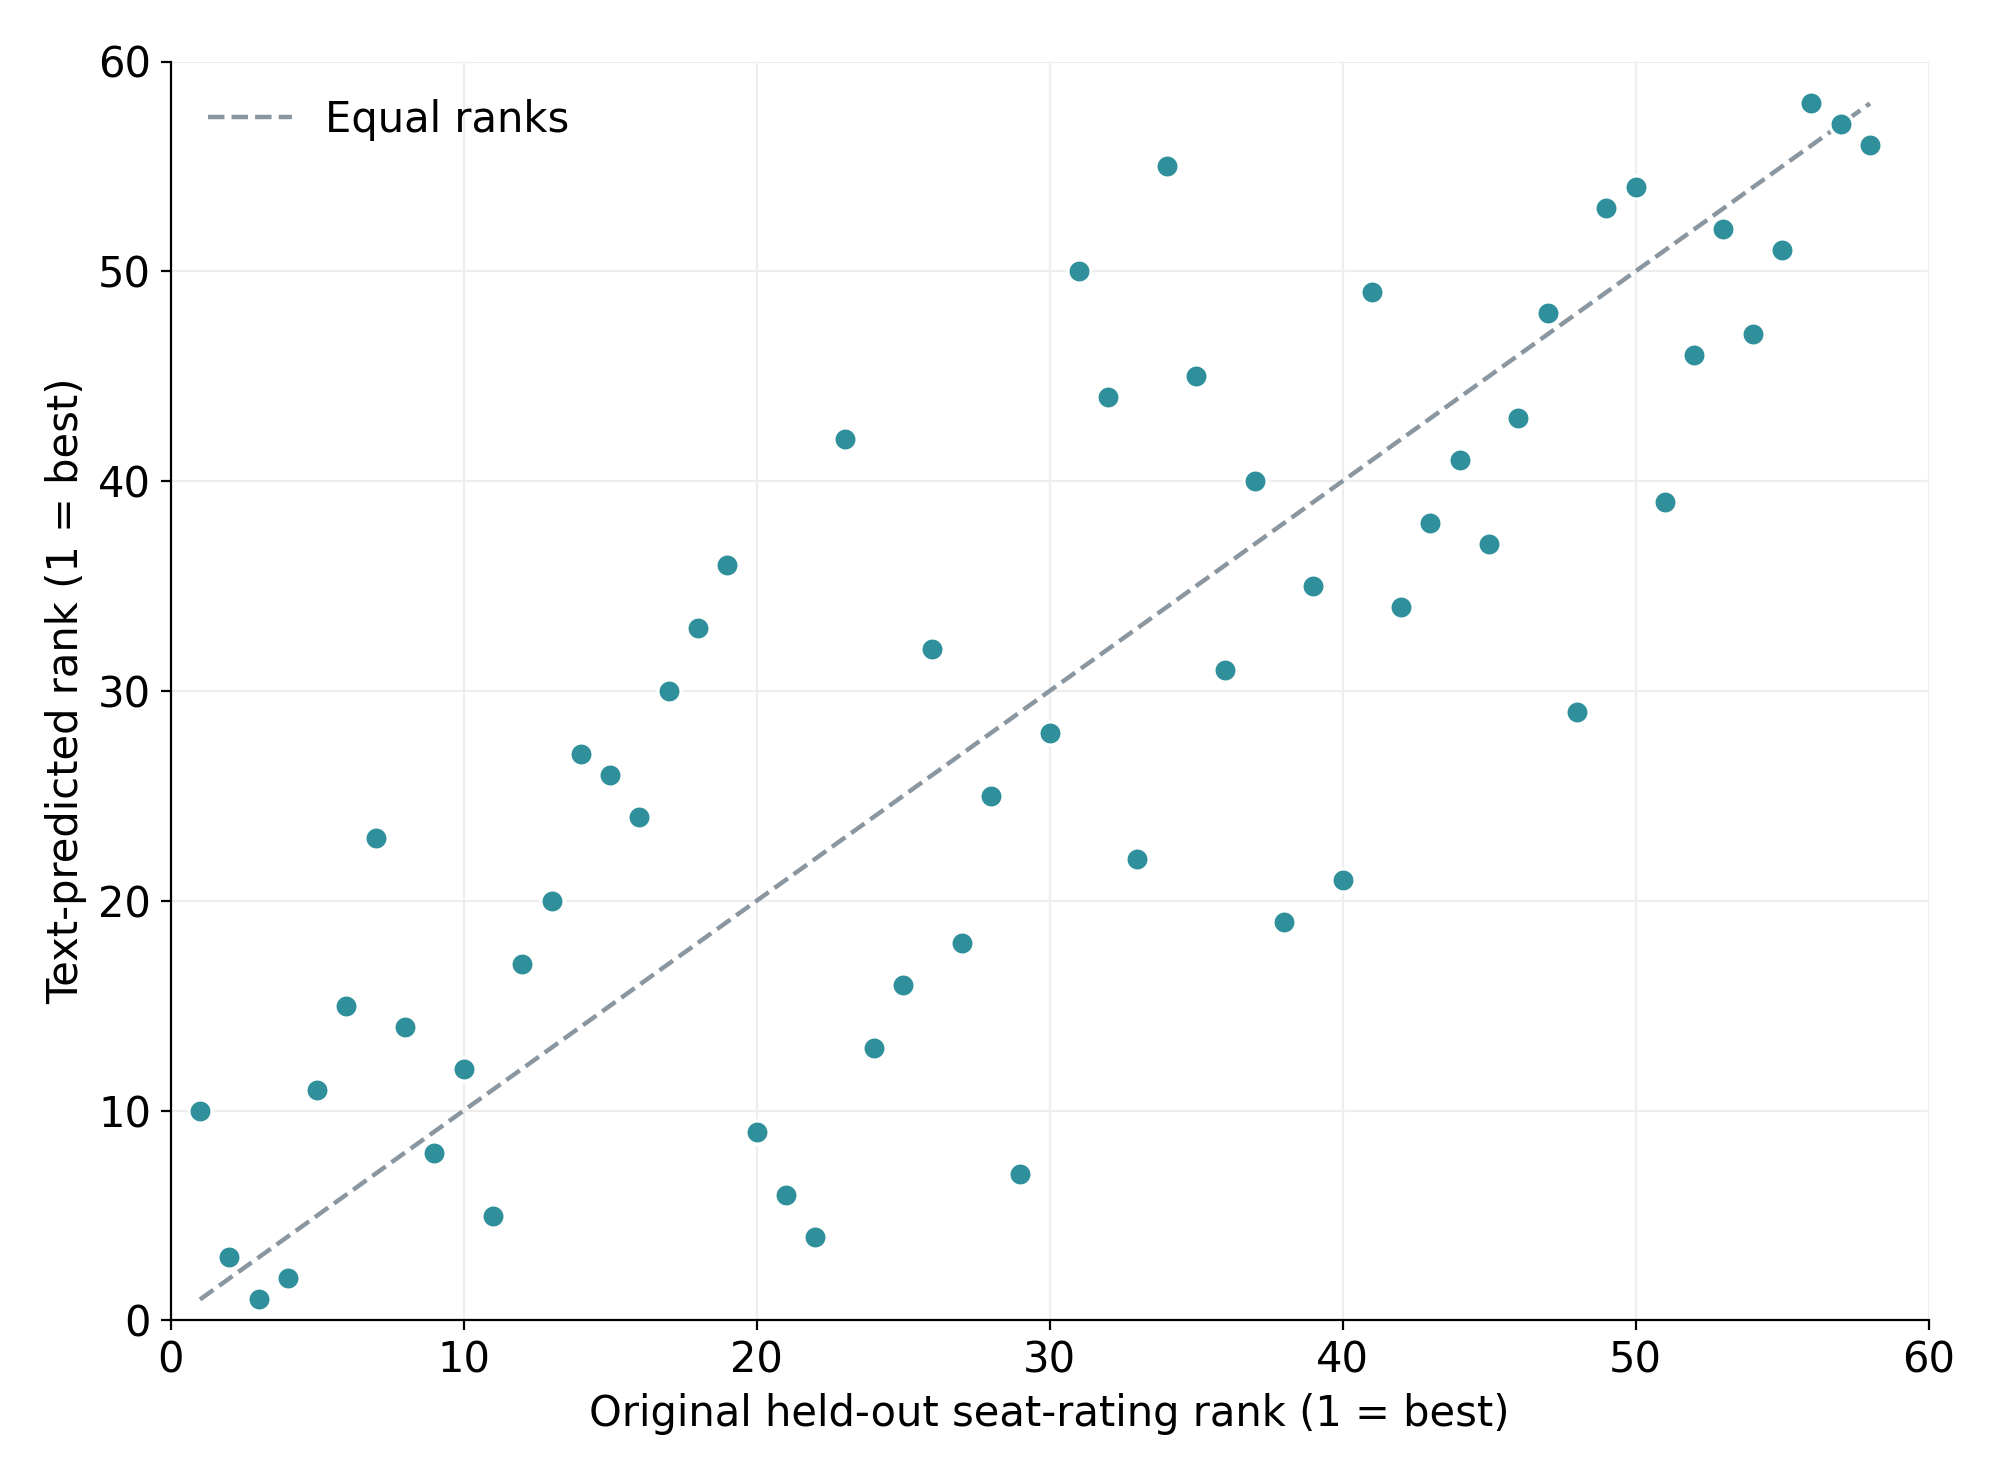
\includegraphics[width=\columnwidth, ]{figures/airline_rank_agreement.png}
\caption{E7：58 家航司的文本预测名次与留出评分名次（1 为最好）；虚线表示名次相同。Spearman $\rho=0.806$，95\% 区间 $[0.675, 0.833]$。}
\label{fig:rank}
\end{figure}

\paragraph{结果。}共有 58 家航司达到门槛。留出的参照集中有 \num{8365} 条有有效座椅评分的评论，其中 \num{3154} 条有可用的文本预测。两份排名高度一致：Spearman $\rho=0.806$，95\% 区间 $[0.675,0.833]$，区间来自在固定航司集合上对父评论做 2,000 次配对重采样（图~\ref{fig:rank}）。可见从文本中挖掘并按评论聚合的观点，保留了航司之间的明显差异，这支持用评论文本回答比较类问题。评分是整体座椅舒适度的参照，并不是每个细分属性的标准答案；区间也不包含重新训练分类器带来的不确定性。

\subsection{E8：性能与可扩展性（Q4）}
\label{sec:exp-perf}

\begin{table}[t]
\centering\small
\caption{E8：Apple M1 Pro（16\,GB）上的性能。查询耗时为 20 个评估问题的中位数（P95）。}
\label{tab:perf}
\setlength{\tabcolsep}{3pt}
\begin{tabularx}{\columnwidth}{@{}Yr@{}}
\toprule
\textbf{指标} & \textbf{数值} \\
\midrule
检索与证据挑选 & 2.9\,s（10.5\,s） \\
提交到首个流式字符 & 24.3\,s（41.9\,s） \\
提交到最终校验通过的回答 & 40.8\,s（72.3\,s） \\
仅程序回答（关闭 LLM） & 5.0\,s / 次 \\
短 LLM 请求（120 token），同时 1 或 2 个 & 每个 $\approx$1\,s，串行处理 \\
\midrule
学生模型标注 \num{529031} 句 & 18\,s \\
一次性 MiniLM 编码全部句子 & 573\,s \\
LLM 教师标注 & $\approx$0.5\,s / 句 \\
知识库重建 / BM25 构建 / FAISS 构建 & 14\,min / 6\,s / 4.6\,min \\
\midrule
每次查询成本 & \$0（全部本地） \\
\bottomrule
\end{tabularx}
\end{table}

检索和打标的可扩展性很好：索引和标签离线构建，查询耗时取决于过滤后的子集，而不是语料总量；学生模型每秒约标注 \num{30000} 句（表~\ref{tab:perf}）。瓶颈在生成。我们只有一个 MLX 服务，一次只处理一个请求，两个用户同时提问时等待时间大约翻倍；要服务更多用户，需要多个模型实例，或在 GPU 服务器上用 vLLM 这类批处理推理引擎。5\,s 的纯程序路径可以在高负载时作为后备。

%--------------------------------------------------------------- 讨论
\section{讨论与局限}
\label{sec:disc}

\paragraph{自动评判。}检索相关性和 RAG 指标都是自动的，RAG 评判者就是生成器本身。在 E6 中评判者给所有回答的相关性都打了满分，这个指标没有提供信息；上下文精确率在展示相同片段的配置之间也会变动，因为评判者打分时能看到回答。bootstrap 区间无法反映这类评判误差。人工相关性判断和隐藏配置名称的人工审阅回答（最好再换一个独立的评判模型）会让 E1、E5、E6 更有说服力。

\paragraph{生成模型太小，校验偏严。}E5 的 20 个回答中有 16 个、E6 中开启 Z 的 80 个回答中有 62 个用了程序生成的后备回答，E6 被拒的 64 份初稿中有 22 份只是格式不合格。反过来，Q01 的一份初稿把“98 条有明确倾向的评论”写成“98 条正面评论”（实际为 78 条），数字校验因为 98 是允许出现的数值而放过了它，这份初稿只是因为格式问题才被拒绝。下一步应区分语义错误和格式违规，并测量误拒率；更大的本地模型，或在通过校验的回答上做小规模微调，也会有帮助。

\paragraph{分类器未达目标。}方面 F1 为 70.4，目标是 85。由于教师标签的单位价值高于弱标签，成本最低的下一步是：更多教师标签（3--5 万句，GPU 上几小时）、在其上微调一个小编码器，以及只把低置信度句子送给 LLM 的级联方案。允许一句话标多个方面也会更符合数据。

\paragraph{英文航司名。}后期测试发现 “\ldots Cathay Pacific or Singapore Airlines?” 被解析成单航司问题，原因是语料里的写法是 “Cathay Pacific Airways”。现已加入常用英文简称对照表解决（不改变任何评估问题的解析结果）；表外的名称仍需使用语料中的写法、中文名或侧栏。

\paragraph{数据时效。}评论截至 2019 年年中。界面在每一页都注明了这一点；回答描述的是历史体验，而非当前服务。

%--------------------------------------------------------------- 结论
\section{结论}

我们构建了一个本地运行的航空服务问答 RAG 系统，它遵守约束、能细到具体属性，并给出用户可核对的结论。有四点体会最深。第一，结构化约束和属性路由修好了表~\ref{tab:fixes} 中的失败查询：仅元数据硬约束就让 NDCG@10 提高 0.76（E1b），远超更换排序模型带来的变化，通用交叉编码器甚至起了反作用。第二，把 LLM 标注器蒸馏成线性分类器，能以极小的成本拿到它在客观句识别上的大部分收益和联合准确率上约一半的收益，前提是模型选择远离测试集。第三，带程序后备的校验给出最忠实的最终回答（仅 Z 是八种配置中最好的），但各组件的收益并不可加：精确的全量统计修好了结论，却拉低了评判出的忠实度；而且在 4B 生成模型下，Z 的收益大部分来自用程序文字替换模型文字。最后，从文本挖掘出的航司排名与留出的乘客评分高度一致（$\rho=0.81$），这支持用评论文本回答比较类问题。

%--------------------------------------------------------------- 附属信息
\section*{数据与代码获取}

\textbf{Release 页面：}\url{https://github.com/ntu-ai6127-g-13/ai6127-airline-rag/releases/tag/v1.0-submission}

\textbf{数据压缩包：}\url{https://github.com/ntu-ai6127-g-13/ai6127-airline-rag/releases/download/v1.0-submission/ai6127-g13-data.zip}\\
\nolinkurl{chunks.parquet}（知识库）、\texttt{eval.xls} 及冻结的 gold CSV、20 个评估问题的检索证据与生成回答、30 个查询的检索基准及逐查询结果、标签索引（v4.1 与蒸馏版）、gold 上的分类预测、教师标签、消融案例文件、析因消融的完整运行记录（协议、提示词、160 条回答、评判分数），以及航司排名预测。

\textbf{代码压缩包：}\url{https://github.com/ntu-ai6127-g-13/ai6127-airline-rag/archive/refs/tags/v1.0-submission.zip}\\
\nolinkurl{src/}、\nolinkurl{app/}、\nolinkurl{scripts/}、\nolinkurl{experiments/}、\nolinkurl{tests/}、\nolinkurl{requirements.txt}，以及说明如何构建和运行的 README。

\section*{贡献声明}
所有成员都参与了项目。按作业说明的推荐做法，我们申请全组共享同一个成绩。

\printbibliography

%--------------------------------------------------------------- 附录
\appendix
\onecolumn
\section{复现实验结果}
\label{app:repro}

所有命令都在仓库根目录下用 Python 3.11 运行。实验脚本不会覆盖已有结果：多数脚本拒绝写入已存在的输出目录，耗时长的脚本则从检查点续跑；蒸馏相关脚本还会记录输入文件的 SHA-256 哈希。

\begin{Verbatim}[fontsize=\footnotesize, frame=single, framesep=3mm, rulecolor=\color{black!25}]
# environment and data (Q1)
python3.11 -m venv .venv && .venv/bin/pip install -r requirements.txt
.venv/bin/python -m spacy download en_core_web_sm
.venv/bin/python scripts/download_data.py
.venv/bin/python -m src.build_kb                       # about 14 min

# indexes
.venv/bin/python -m src.retriever build-bm25
.venv/bin/python -m src.retriever build-dense --batch-size 64
.venv/bin/python -m src.label_index --model outputs/weak_rebuild_20261019/model.joblib \
    --output-dir outputs/label_index_replay     # the archive already has label_index_20261019

# interface (Q2): local model server, then the app
.venv/bin/python scripts/setup_query_model.py           # once: pinned Qwen3-4B weights
outputs/query_quality_runtime/venv311/bin/python scripts/local_qa_server.py
.venv/bin/python scripts/run_query_app.py --port 8517

# retrieval benchmark and targeted checks (E1, E6); RAG metrics and latency (E2, E5)
.venv/bin/python -u experiments/final_auto_eval/run.py --output-dir outputs/final_auto_eval_replay
.venv/bin/python -u experiments/final_rag_eval/run.py --output-dir outputs/final_rag_eval_replay
# retrieval innovation ablation (E1b); the LLM judge needs the model server running
.venv/bin/python -u experiments/final_auto_eval/retrieval_ablation.py \
    --output-dir outputs/retrieval_ablation_replay

# factorial ablation (E6; needs the model server) and airline ranking (E7);
# details in experiments/downstream_evaluation/README.md
.venv/bin/python -u experiments/downstream_evaluation/factorial.py \
    --output-dir outputs/q5_factorial_replay
P=outputs/downstream_protocol_replay
.venv/bin/python -m experiments.downstream_evaluation.freeze --output-dir $P
.venv/bin/python -m experiments.downstream_evaluation.ranking \
    --protocol $P/protocol.json --output-dir outputs/downstream_ranking_replay

# distillation (E3, E4); encode.py and evaluate_gold.py default to --device mps (use cpu/cuda
# elsewhere). The teacher step needs the MLX runtime and earlier r36 outputs, so the sample and
# its teacher labels ship in the data archive ($S); sample.py and label_teacher.py remake them.
D=experiments/distilled_label_index; O=outputs
S=$O/distill_sample_20261029; E=$O/distill_embeddings_20261029; R=$O/distill_students_replay
.venv/bin/python $D/encode.py --output-dir $E                                   # 5-10 min
.venv/bin/python $D/train_students.py --sample-dir $S --embeddings $E --output-dir $R
.venv/bin/python $D/evaluate_gold.py --selection $R/selection.json --output-dir $R/gold
.venv/bin/python $D/build_index.py --audit $R/gold/gold_audit.json \
    --selection $R/selection.json --embeddings $E --output-dir $O/label_index_distilled_replay
\end{Verbatim}

\section{评估文件格式}
\label{app:eval}

\texttt{eval.xls}（SHA-256 \texttt{fe0bcf0c…a477045}）是用 \texttt{xlwt} 从冻结的 gold CSV 写出的 Excel 97--2003 工作簿：一个工作表，共 \num{1000} 行，无重复文本，只有基准格式要求的 \texttt{text} 和 \texttt{label} 两列。gold CSV（\nolinkurl{data/eval/gold_human_frozen_1000_20261019_v1.csv}）行与顺序相同，另含分步标签和来源信息：

\begin{center}\small
\begin{tabularx}{\textwidth}{@{}P{34mm}P{52mm}Y@{}}
\toprule
\textbf{列} & \textbf{取值} & \textbf{含义} \\
\midrule
\texttt{text} & 字符串 & 句子原文，与标注者看到的完全一致。 \\
\texttt{label} & objective / positive / negative & 三分类情感标签（基准格式）。 \\
\texttt{subjectivity} & objective / subjective & 任务第一步。 \\
\texttt{polarity} & positive / negative / NA & 任务第二步；客观句为 \texttt{NA}（读取时用 \nolinkurl{keep_default_na=False}）。 \\
\texttt{aspect} & seat, staff, food, entertainment, ground, value, overall, other & 句子所谈的方面。 \\
ID 与来源信息 & 句子、评论和切块 ID；审核状态 & 可回连知识库；人工审核的记录。 \\
\bottomrule
\end{tabularx}
\end{center}

\paragraph{问题集。}\nolinkurl{data/eval/query_smoke_40_20261019.json} 是一个含 40 个问题的 JSON 数组，每题有 \texttt{id}、\texttt{language}、\texttt{question}、预期的 \texttt{aspect}/\texttt{aspects}、预期的 \texttt{subtopics}（细分属性）和 \texttt{comparison} 标记。E1 把 Q01--Q25 解析为 30 个“航司 $\times$ 细分属性”单元；E2 和 E5 使用 Q01--Q12、Q21--Q25 和 Q28--Q30。结果为每题一条记录的 JSONL（\texttt{case}、\texttt{parsed}、含检索证据和耗时的 \texttt{result}、含文本/来源/引用的 \texttt{answer}，以及 \texttt{judge}），或每个查询和方法一行的 CSV。

\section{表~\ref{tab:five} 中的查询：原文与结果}
\label{app:queries}

计数为直接匹配该属性的评论；百分比以其中有明确倾向的评论为分母。完整回答（含引用和证据）见
\nolinkurl{outputs/final_rag_eval_20261019/answers.jsonl}。

\begin{center}\small
\begin{tabularx}{\textwidth}{@{}lP{62mm}Y@{}}
\toprule
\textbf{编号} & \textbf{提问原文} & \textbf{结果} \\
\midrule
Q05 & 阿联酋航空经济舱的退款和改签处理怎么样？ & 负面：19 条有倾向的评论全部负面（共 24 条匹配）；引用了多次联系仍未退款、取消费和选座费等。 \\
Q10 & 卡塔尔航空商务舱的电影选择和娱乐内容怎么样？ & 两极：15 正、15 负（86 条匹配）；片库丰富与内容陈旧、电视节目少并存。 \\
Q24 & 国泰航空和新加坡航空经济舱腿部空间哪家评价更好？ & 腿部空间无明确胜者：国泰 72.5\% 正面（50/69），新航 79.6\%（78/98）；新航座椅评分更高（3.83 对 3.46）。 \\
Q28 & 新加坡航空经济舱的腿部空间、靠背调节、座椅舒适度和座椅清洁度分别怎么样？ & 腿部空间偏正面（78/98，79.6\%）；靠背调节两极（14/26）；座椅舒适度偏正面（97/123，78.9\%）；清洁度样本太少（7/10）。 \\
Q30 & 新加坡航空经济舱的餐食、性价比和地面服务分别怎么样？ & 餐食 65.5\% 正面（289/441，评分 3.88）；性价比 34.6\% 正面（75/217，评分 3.88）；地面服务 43.6\% 正面（163/374，评分 3.99）。 \\
\bottomrule
\end{tabularx}
\end{center}

\section{析因消融使用的问题}
\label{app:factorial}

每题的问法为 “What do historical reviews say about [attribute] on [airline] in [cabin]?”。下表属性为中文意译，英文原句见数据包中的 \texttt{outputs/q5\_factorial\_20261104/protocol.json}。这里的编号只在 E6 内使用，与表~\ref{tab:five} 的编号无关。

\begin{center}\small
\begin{tabular}{@{}llll@{\hspace{10mm}}llll@{}}
\toprule
\textbf{ID} & \textbf{航司} & \textbf{舱位} & \textbf{属性} & \textbf{ID} & \textbf{航司} & \textbf{舱位} & \textbf{属性} \\
\midrule
Q01 & Singapore Airlines & 经济舱 & 腿部空间 & Q11 & British Airways & 超级经济舱 & 靠背调节与平躺 \\
Q02 & Air Canada rouge & 经济舱 & 腿部空间 & Q12 & Cathay Pacific & 商务舱 & 空乘态度 \\
Q03 & Spirit Airlines & 经济舱 & 行李服务 & Q13 & United Airlines & 经济舱 & 座椅宽度 \\
Q04 & Alaska Airlines & 经济舱 & 延误与取消处理 & Q14 & Turkish Airlines & 经济舱 & 餐食品质与口味 \\
Q05 & Emirates & 经济舱 & 退改签 & Q15 & AirAsia & 经济舱 & 客服 \\
Q06 & Singapore Airlines & 经济舱 & 餐食种类 & Q16 & Etihad Airways & 商务舱 & 靠背调节与平躺 \\
Q07 & Singapore Airlines & 经济舱 & 餐食分量 & Q17 & Frontier Airlines & 经济舱 & 行李服务 \\
Q08 & Singapore Airlines & 经济舱 & 座椅清洁度 & Q18 & American Airlines & 经济舱 & 值机服务 \\
Q09 & Emirates & 经济舱 & 机上 Wi-Fi & Q19 & Lufthansa & 经济舱 & 准点表现 \\
Q10 & Qatar Airways & 商务舱 & 娱乐内容 & Q20 & Qantas Airways & 经济舱 & 机上饮品 \\
\bottomrule
\end{tabular}
\end{center}

\section{方面与细分属性分类体系}
\label{app:taxonomy}

\begin{center}\small
\begin{tabularx}{\textwidth}{@{}P{30mm}Y@{}}
\toprule
\textbf{方面} & \textbf{细分属性（共 46 个）} \\
\midrule
座椅 & 腿部空间、宽度、靠背调节与平躺、舒适度、座椅状况、座椅清洁度、电源、私密性、储物 \\
餐食 & 具体菜品、品质与口味、分量、多样性、饮品、特殊餐、温度、餐饮服务流程 \\
娱乐 & 内容、屏幕、Wi-Fi、耳机与音频、系统易用性 \\
员工 & 态度、效率、专业性、响应及时性、沟通与语言 \\
地面 & 准点、延误与取消处理、行李、值机、登机口与登机、贵宾室、中转、特殊协助 \\
性价比 & 票价、退改签、客服、订票系统、附加费用 \\
其他 & 客舱清洁、洗手间、客舱温度、洗漱用品、客舱噪音、飞机与客舱状况 \\
总体 & 对整趟行程的评价；无细分属性 \\
\bottomrule
\end{tabularx}
\end{center}

\end{document}
